\documentclass[12pt,a4paper,english
% ,twoside,openright
]{tunithesis}

% Note that you must choose either Finnish or English here and there in this
% file.
% Other options for document class
  % ,twoside,openright   % If printing on both sides (>80 pages)
  % ,twocolumn           % Can be used in lab reports, not in theses

% Ensure the correct Pdf size (not needed in all environments)
\special{papersize=210mm,297mm}


% LaTeX file for BSC/MSc theses and lab reports.
% Requires the class file (=template) tunithesis.cls and figure files,
% either tut-logo, exampleFig (as pdf or eps) and example_code.c
% Author: Lucas Machado (2018)
% Based on TTU template by Sami Paavilainen (2006), modified by Heikki Huttunen (2014)

% More information about Latex basics:
% [Tobias Oetiker, Hubert Partl, Irene Hyna, Elisabeth Schlegl, The
% Not So Short Introduction to LATEX2e, Version 5.03, April 2014, 171
% pages.  Availbale: http://tobi.oetiker.ch/lshort/lshort.pdf]

\author{Väinö-Waltteri Granat}
%\title{Zero to DLA: Building Software Support For Custom RISC-V SoC To Accelerate Deep Neural Networks} % primary title (for front page)
\title{Zero to DLA: Building a Software Stack for Accelerating Deep Neural Networks on Custom RISC-V SoC} % primary title (for front page)
\def\finnishtitle{Ohjelmistopinon kehittäminen syväoppivien neuroverkkojen kiihdyttämiseksi mukautetulla RISC-V järjestelmäpiirillä}
\thesistype{Master of Science Thesis} % or Bachelor of Science, Laboratory Report...

% Put your thesis' main language last
% http://mirrors.ctan.org/macros/latex/required/babel/base/babel.pdf
\usepackage{lastpage}
\usepackage[english]{babel}
\usepackage[
backend=biber,
style=numeric-comp,
citestyle=numeric-comp,
autocite=footnote,
maxbibnames=5
]{biblatex}
\usepackage{csquotes}
\usepackage{booktabs}
\usepackage{adjustbox}
\usepackage{subcaption}
\usepackage{caption}
\usepackage{svg}
\usepackage[withpage]{acronym}
\usepackage{tikz}
\usetikzlibrary{arrows.meta, arrows}
\usetikzlibrary{matrix, positioning}
\usepackage{xcolor}
\usepackage{amsfonts}
\usepackage{listings, listings-rust}
%\usepackage{inconsolata}
\usepackage{graphicx}
\usepackage{float}
\usepackage{multirow}
\usepackage{calc}

\addbibresource{thesis_refs.bib} %Imports bibliography file
\addbibresource{zotero.bib} %Imports bibliography file

% Table caption on top
\floatstyle{plaintop}
\restylefloat{table}

% Fix this
\newcommand{\fixthis}[1]{\textbf{\textit{\textcolor{red}{[#1]}}}}

\definecolor{tunipurple}{RGB}{78, 0, 142}

%\hyphenation{jär-jes-tel-mä-pii-re-jä}

\newcommand\todo[1]{{\color{red}!!!TODO: #1}} % Remark text in braces appears in red
\newcommand{\angs}{\textsl{\AA}}              % , e.g. slanted symbol for Ångstöm
\def\checkmark{\tikz\fill[scale=0.4](0,.35) -- (.25,0) -- (1,.7) -- (.25,.15) -- cycle;}
\def\scalecheck{\resizebox{\widthof{\checkmark}*\ratio{\widthof{x}}{\widthof{\normalsize x}}}{!}{\checkmark}}
\lstdefinestyle{customc}{
  belowcaptionskip=1\baselineskip,
  breaklines=true,
  frame=L,
  xleftmargin=\parindent,
  language=C,
  showstringspaces=false,
  basicstyle=\footnotesize\ttfamily,
  keywordstyle=\bfseries\color{green!40!black},
  commentstyle=\itshape\color{purple!40!black},
  identifierstyle=\color{blue},
  stringstyle=\color{orange},
  postbreak=\mbox{\textcolor{red}{$\hookrightarrow$}\space},
}

\lstdefinestyle{customasm}{
  belowcaptionskip=1\baselineskip,
  frame=L,
  xleftmargin=\parindent,
  language=[x86masm]Assembler,
  basicstyle=\footnotesize\ttfamily,
  commentstyle=\itshape\color{purple!40!black},
}

\lstset{escapechar=@,style=customc}

\pagenumbering{roman} % was: {Roman}
\pagestyle{headings}
\begin{document}

% Special trick so that internal macros (denoted with @ in their name)
% can be used outside the cls file (e.g. \@author)
\makeatletter

\thispagestyle{empty}
\vspace*{-.5cm}\noindent

\begin{figure}
    \vspace{-1.3cm}
    \advance\leftskip-2.5cm
    \noindent
\includegraphics{img/tunilogo.png}
\end{figure}
 
\vspace{2.5cm}
\begin{flushright}
\noindent\textsf{\LARGE{\@author}}

\noindent\vspace{0.5cm}

\noindent\Huge{\textsf{\textbf{\textcolor{tunipurple}{\@title}}}}
\end{flushright}
\vspace{10.7cm} % adjust to 12.7 this if thesis title needs two lines

% Last some additional info to the bottom-right corner
\begin{flushright}  
    \begin{spacing}{1.0}
      \textsf{Faculty of Information Technology and Communication Sciences (ITC)\\
      \@thesistype\\
      November 2024}
    \end{spacing}
\end{flushright}

% Leave the backside of title page empty in twoside mode
\if@twoside
\clearpage
\fi


% Turn off page numbering for the first pages
\pagenumbering{gobble}

\chapter*{Abstract}

\begin{spacing}{1.0}
\noindent \@author: \@title\\
\@thesistype\\
Tampere University\\
Master’s Degree Programme in Information Technology\\
November 2024
\end{spacing}
\noindent\rule{12cm}{0.4pt}

\vspace{0.5cm}

% ---------------------------------------
% Abstract and keywords
% ---------------------------------------

\noindent In recent years we have seen a large increase in the number of applications utilizing convolutional neural networks on mobile device in our everyday-life. This phenomenon has coincided with the increased interest in heterogeneous system-on-chips in consumer electronics. This has motivated organizations and research groups to build their own SoCs. One such SoC is Headsail. A multicore RISC-V SoC featuring a variety of peripherals, developed in Tampere University's SoC Hub research team.

The purpose of this project was to target Headsail's custom deep learning accelerator, and develop a software stack to utilize its capabilities for running inference on arbitrary convolutional neural networks. At the time of starting this project Headsail was still in development so we built a Headsail virtual prototype with the accelerator using Renode, and Renode's Python peripheral API. The goal was to run a neural accelerator benchmark simulating real-life use cases on the virtual prototype to confirm the feasibility of the stack, and then to run the same use case on the ASIC.
This necessitated for us to develop a driver for the accelerator, BSP for the platform and port a C standard library for it, integrate the platform package with the TVM machine learning compiler and finally to evaluate the accuracy of the stack and the accelerator.

In the end we were able to design and build a working software stack to facilitate the SoC aswell as the deep learning accelerator. We were also able to integrate the stack with TVM, which enabled us to build programs to run inference on quantized convolutional neural network, trained on common high-level deep learning framework. Using MLPerf Tiny benchmark we were able to evaluate the accuracy of the stack and concluded that DLA is capable of executing some models with an acceptable accuracy. Due to time constraints we were not able to run the benchmark on the final ASIC.

\noindent\textbf{Keywords:} deep learning, system-on-chip, RISC-V, TVM, Renode, MLPerf Tiny

~

\noindent The originality of this thesis has been checked using the Turnitin Originality Check service.


\clearpage

\chapter*{Tiivistelmä}

\begin{spacing}{1.0}
\noindent \@author: \finnishtitle\\
Diplomityö\\
Tampereen yliopisto\\
Tietotekniikan diplomi-insinöörin tutkinto-ohjelma \\
Marraskuu 2024
\end{spacing}
\noindent\rule{12cm}{0.4pt}

\vspace{0.5cm}

% ---------------------------------------
% Abstract and keywords
% ---------------------------------------

\noindent \foreignlanguage{finnish}{Arkielämässämme kohtaamiemme konvolutioverkkoja hyödyntävien sovellusten mää\-rä on lisääntynyt, samanaikaisesti kiinnostuksen kasvaessa heterogeenisiä jär\-jes\-tel\-mä\-pii\-re\-jä kohtaan. Yksi esimerkki tällaisesta järjestelmäpiiristä on Tampereen yliopiston SoC Hub -tutkimusryhmässä kehitetty Headsail. Headsailissä on avoimeen RISC-V -suoritinarkkitehtuuriin pohjautuva moniydinsuoritin, joka sisältää useita
oheislaitteita, joista yksi on syväoppimiskiihdytin.}

\foreignlanguage{finnish}{Työn tarkoituksena oli suunnitella ohjelmistopino jolla sy\-vä\-op\-pi\-mis\-kiih\-dy\-tin\-tä voi\-tai\-siin käyttää päätelmien laskemiseen.
Projektin alkaessa Headsail oli vielä kehityksessä, joten rakensimme sitä vastaanvan virtuaaliprototyypin, jossa oli mukana myös syväoppimiskiihdytin. Virtuaaliprototyyppi rakennettiin Renode-alustaa ja sen Python-oheislaiterajapintaa hyödyntäen. Tavoitteena oli suorittaa sellainen suorituskykytesti, joka mukailisi neuroverkkojen todellisia käyttötapauksia, siten että ohjelmistopinon soveltuvuus voitaisiin varmistaa. Lopuksi sama testi suoritettaisiin myös lopullisella piirillä. Tähän tarkoitukseen kehitimme ainakin seuraavat komponentit: ajurin syväoppimiskiihdyttimen käyttöä varten, alustakohtaisen tukipaketin ja version C-standardikirjastosta, TVM koneoppimiskääntäjän kanssa yhteensopivan integraation ja lopuksi menetelmän ohjelmistopinon  ja kiihdyttimen arvioimiseksi.}

\foreignlanguage{finnish}{Lopulta saimme valmiiksi syväoppimiskiihdyttimen käytön mahdollistavan ohjelmistopinon. Integraatio TVM-koneoppimiskääntäjän kanssa, mahdollisti sellaisten ohjelmistojen kehittämisen, joissa hyödynnettiin korkeantason alustoilla kehitettyjä kvantisoituja konvoluutioneuroverkkoja. MLPerf Tiny -suorituskykytestin avulla pystyimme arvioimaan ohjelmistopinoa hyödyntävien ohjelmistojen ennustustarkkuuden ja osoittamaan että Headsailin syväoppimiskiihdytintä voidaan käyttää kiihdyttmään joitain neuroverkkoja, siten että tarkkuus säilyy hyväksyttävänä. Aikarajoitteiden vuoksi emme kuitenkaan pystyneet suorittamaan samaa testiä lopullisella piirillä.}


\noindent\textbf{Keywords:} syväoppiminen, järjestelmäpiiri, RISC-V, TVM, Renode, MLPerf Tiny

~

\noindent Tämän julkaisun alkuperäisyys on tarkastettu Turnitin OriginalityCheck -ohjelmalla.


\clearpage

\clearpage
\chapter*{\@aidisclaimertitle}
Artificial intelligence (AI) has been used in generating this work:


I hereby declare, that the AI-based applications used in generating this work are as follows:

\begin{center}
    \begin{tabular}{c|l}
        \toprule
        \textbf{Application} & \textbf{Version} \\
        \midrule
        OpenAi, ChatGPT-4 Turbo & April - November 2024 \\
        Microsoft Copilot & April - November 2024 \\
        \bottomrule
    \end{tabular}
\end{center}

\section*{Purpose of the use of AI}

Large language models were use as an aid for generating code for some of the Tikz diagrams presented in this thesis, with the purpose of improving the quality of the given diagrams.

Explain here \emph{in detail}, for which purpose and how AI was utilized in writing this thesis.

\section*{Parts of this work, where AI was used}

List here all chapters, sections, subsections, tables, figures and so forth,
that were generated by an AI, or that an AI had a hand in generating.

The following figures were created with a help of AI: \ref{fig:rgb-array}, \ref{fig:activation-functions}, \ref{fig:network-simple}, \ref{fig:network-residual}

\section*{Acknowledgement of risks}

I hereby acknowledge, that as the author of this work, I am fully
responsible for the contents presented in this thesis. This includes
the parts that were generated by an AI, in part or in their entirety. I
therefore also acknowledge my responsibility in the case, where use of
AI has resulted in ethical guidelines being breached.

\clearpage


\preface{preface.tex}{Tampere, 29th November 2024}

% TOC
\setcounter{tocdepth}{3}              % How many header level are included
\tableofcontents                      % Create TOC
\clearpage


\section*{List of Abbreviations}
\begin{acronym}
  \acro{AD}{Anomaly Detection}
  \acro{AI}{Artificial Intelligence}
  \acro{AOT}{Ahead-of-Time}
  \acro{API}{Application Programming Interface}
  \acro{ASIC}{Application Specific Integrated Circuit}
  \acro{AUC}{Area Under The Curve}
  \acro{BSP}{Board Support Package}
  \acro{BYOC}{Bring Your Own Codegen}
  \acro{CHW}{Channel Height Width}
  \acro{CI/CD}{Continuous Integration Continuous Delivery}
  \acro{CLINT}{Core Local Interrupt Controller}
  \acro{CNN}{Convolutional Neural Network}
  \acro{CPU}{Central Processing Unit}
  \acro{DL}{Deep Learning}
  \acro{DLA}{Deep Learning Accelerator}
  \acro{DNN}{Deep Neural Network}
  \acro{FFI}{Foreign Function Interface}
  \acro{FIFO}{First In, First Out}
  \acro{FN}{False Negative}
  \acro{FP32}{32-bit Floating Point}
  \acro{FP8}{8-bit Floating Point}
  \acro{FPR}{False Positive Rate}
  \acro{FP}{False Positive}
  \acro{GDB}{GNU Project Debugger}
  \acro{HPC}{High Performance Core}
  \acro{HWC}{Height Width Channel}
  \acro{IC}{Image Classification}
  \acro{INT8}{8-bit Integer}
  \acro{ISA}{Instruction Set Architecture}
  \acro{KWS}{Keyword Spotting}
  \acro{LSB}{Least Significant Bit}
  \acro{MAC}{Multiply-Accumulate}
  \acro{MCU}{Microcontroller Unit}
  \acro{ML}{Machine Learning}
  \acro{MPL}{Multilayer Perceptron}
  \acro{MSB}{Most Significant Bit}
  \acro{PLIC}{Peripheral Level Interrupt Controller}
  \acro{QNN}{Quantized Neural Network}
  \acro{RGB}{Red Green Blue}
  \acro{RTL}{Register Level Transfer}
  \acro{SPI}{Serial Peripheral Interface}
  \acro{SoC}{System on a chip}
  \acro{TN}{True Negative}
  \acro{TPR}{True Positive Rate}
  \acro{TP}{True Positive}
  \acro{UART}{Universal Asynchronous Receiver Transmitter}
  \acro{VP}{Virtual Prototype}
  \acro{VWW}{Visual Wake Words}
\end{acronym}


\thispagestyle{empty}
\listoffigures
\listoftables
\clearpage


% The actual text begins here and page numbering changes to 1,2...
% Leave the backside of title empty in twoside mode
\if@twoside
%\newpage
\cleardoublepage
\fi


\renewcommand{\chaptername}{} % This disables the prefix 'Chapter' or
                              % 'Luku' in page headers (in 'twoside'
                              % mode)


\chapter{Introduction}
\label{ch:introduction}
\pagenumbering{arabic}
\setcounter{page}{1} % Start numbering from zero because command
                     % 'chapter*' does page break

In recent years neural network based applications have become more prominent in our everyday-life, where most smartphones come equipped with predictive text keyboards, facial recognition functionalities and automatic enhancements on pictures. A large driver for this has been the adoption of efficient accelerators in mobile device, that have enabled executing inference on more complex deep neural networks on mobile and edge devices.

This interest in neural networks has coincided with the industry's move towards heterogeneous System-on-chip (SoC) solutions being put into consumer and professional electronics, with the goal of improving task specific performance and improving battery life. With SoCs, a single circuit houses multiple different computing elements, such as a CPU, GPU, memory, IO and task specific accelerators.
In addition to commercial SoCs, academic organization have been taping out their own SoC for research purposes. One such SoC is Headsail by the SoC Hub consortium~\cite{keelhaul} in Tampere University.

This thesis has two goals. First is to build a virtual counterpart of the Headsail, to enable firmware development before the tape-out. We want to know if a high-level full system emulator, can be used as a prototyping platform for firmware development for a heterogeneous SoC.
The second goal is to design and develop a software stack capable of utilizing a deep learning accelerator in Headsail for executing inference of arbitrary INT8 quantized neural networks, alongside a use-case application showcasing these capabilities. We propose one such software stack based on completely open-source technologies, which we develop on the virtual counterpart of Headsail.

This thesis consists of six chapters. Chapter~\ref{ch:background} goes over the necessary background information, for understanding the theory behind our approach. Chapter~\ref{ch:methodology} introduces all the relevant technologies used in the stack, with great detail. Chapter~\ref{ch:implementation} present our solution for the described software stack, explains the rationale without design choices. Chapter~\ref{ch:results} presents the results of the benchmark for the virtual version of Headsail. And finally, chapter~\ref{ch:conclusions} is the concluding chapter that summarizes the work presented in this thesis, and presents topics for future work that could be done to improve the work presented in this thesis.

\chapter{Background}
This section covers the topics in Deep Learning that relate to the implementation of the project, with focus on performing inference on deep neural networks. In addition to this we discuss hardware approaches for building tightly integrated single chip systems with SoCs and for accelerating inference workloads with dedicated deep learning accelerators.
\label{ch:background}
\section{Machine Learning}
\begin{figure}
  \centering
  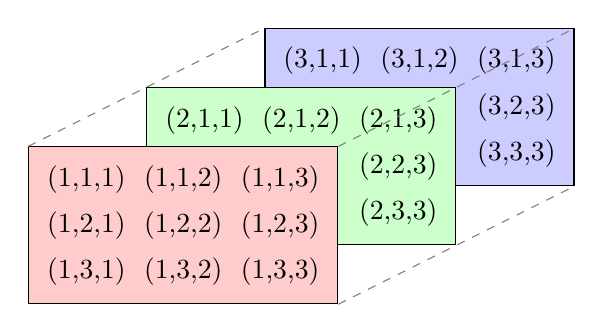
\begin{tikzpicture}
  \def\xs{-1.5} %shift in x direction
  \def\ys{-0.75} %shift in y direction
  \def\nm{3} % number of 2d matrices in the 3d matrix
  \foreach \x in {3,2,1}
  {
      \pgfmathsetmacro\bgcolor{ifthenelse(\x==1,"red!20",ifthenelse(\x==2,"green!20","blue!20"))}

      \matrix [draw, % for the rectangle border
              fill=\bgcolor, % different background colors
              ampersand replacement=\&] % see explanation
      (mm\x)% give the matrix a name
      at(-\x * \xs, -\x * \ys) % shift the matrix
      {
          \node {(\x,1,1)}; \& \node {(\x,1,2)}; \& \node {(\x,1,3)};\\
          \node {(\x,2,1)}; \& \node {(\x,2,2)}; \& \node {(\x,2,3)};\\
          \node {(\x,3,1)}; \& \node {(\x,3,2)}; \& \node {(\x,3,3)};\\
      };
  }

  \draw [dashed,gray](mm1.north west) -- (mm\nm.north west);
  \draw [dashed,gray](mm1.north east) -- (mm\nm.north east);
  \draw [dashed,gray](mm1.south east) -- (mm\nm.south east);
  \end{tikzpicture}
  \caption{RGB array}
  \label{fig:rgb-array}
\end{figure}

Machine Learning is a field of computer science that researches algorithms that allow programs to adapt to given inputs as means to improve itself.~\cite{mitchell1997machine}
The central component of machine learning is the model, which is a function that distinguishes a concept from data.

To build a model we first need training data. Training data is a set of data, often with known associated categories, that corresponds with the unseen data we want to categorize with the model. For example if training a model to count the number of people in image, we would have a training data consisting of images with different amount of people, with the wanted categorization (number of people present in the image) associated with each. This is known as supervised learning, as opposed to unsupervised learning where the class labels are not present. Model is then trained by choosing a particular function and changing its parameters so that it can categorize training data in a wanted manner. After training the performance can then be validated by feeding the model unseen data and seeing how well it can categorize it.

A particular model's domain and codomain are defined by the given problem statement. For example, inputs of an image classifier are three-dimensional arrays, where the second and third dimensions correspond to the height and width of the image and the first dimension as the channel in RGB color space as shown in figure~\ref{fig:rgb-array}, this commonly known as CHW layout.
The output of this model would be one or more labels from the codomain.


\subsection{Function and Model}
In mathematics a function describes the relation between a domain $X$ and codomain $Y$ where
\begin{equation}
  f \subseteq X \times Y,
\end{equation}
meaning that for every element in the domain $X$ there is exactly one corresponding element in codomain $Y$. Using arrow syntax this same mapping is expressed as $f : X \mapsto Y$. If we consider the discovered model as a function, we can view the domain $X$ as the input of a model and codomain $Y$ as the prediction space of the model. For a 10 class classifier codomain $Y$ would be defined as
\begin{equation}
  Y = \{0, 1, 2 ..., 9\}.
\end{equation}

The purpose of a model then, is to map it's input to the codomain in such a manner in which useful information can be acquired from the mapping.
The domain of the network depends on the problem statement. For an image binary classifier $f$ using RGB images as input the formal definition would be the following
\begin{equation}
  f: X \in \mathbb{Z}^{C \times H \times W} \mapsto \{0, 1\}.
\end{equation}
Depending on the problem statement we give the elements in the codomain descriptive labels. For example if the goal of the model was to tell if an image has a person, 0 might be labeled ``\emph{No}'' and 1 labeled as ``\emph{Yes}''. The previous equation abstracts the model into singular function, but developers tend to think models as a series of multiple functions. By dividing the function into multiple consecutive domains and codomains we can get a better understanding what's happening in the model. One model might consist for to consecutive operations $g$ and $h$
\begin{equation}
  h: X \in \mathbb{Z}^{C \times H \times W} \xrightarrow{g}
\begin{bmatrix} v_1 \\ v_2 \\ \vdots \\ v_8 \end{bmatrix}
\in \mathbb{Z}^8 \xrightarrow{f} \{0, 1\}
\end{equation}
where $g$ maps RGB image domain to a codomain of length 8 is acts as the domain for function $h$ which then maps it to domain of the overall function.


\section{Deep Learning}
Deep learning is a subcategory of machine learning that focuses on using deep neural networks as the model. Deep neural networks are a specific case of multilayer perceptrons where there is at least one hidden layer between input and output layer that introduces non-linearity, to the model. DNNs try to solve the problem of choosing a good model for a problem statement, by allowing the developers to discover a suitable function using a training algorithm.

DNN model is weighted graph where nodes are grouped into mostly sequential layers and vertices connect nodes of consecutive layers with simple operations. The vertices hold weights and biases signifying the amount of association between nodes. Essentially what the graph models is, is a N-dimensional space which the non-linear function inhabits, where each of the vertices introduces its own dimension.
This means that increasing the amount of parameters in a model allows it to approximate more complex function, generally increasing the ability to perform more complex tasks.~\cite{sze_efficient_2017}

DNNs differ from other ML methods by their adaptable general architecture that can facilitate problems magnitudes more difficult than traditional methods allow. This ability to solve increasingly more difficult problems come with a cost of needing large amount of computing resource and training data.

\begin{figure}
\centering
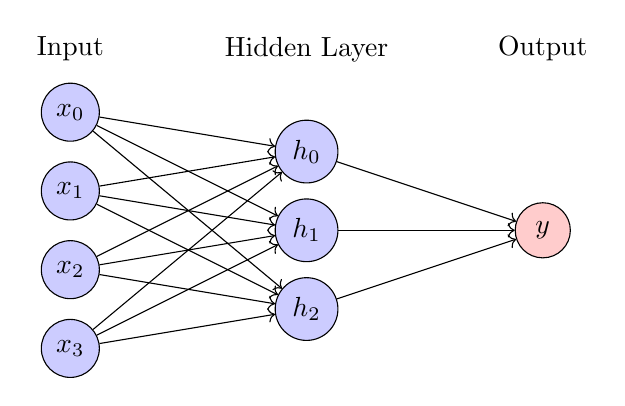
\begin{tikzpicture}
% Input nodes
\node at (0, 1.3) {Input};
\foreach \i in {0, 1, 2, 3} {
  \node[draw, circle, minimum size=0.7cm, fill=blue!20] (input\i) at (0, -\i+0.5) {$x_{\i}$};
}

% Hidden layer nodes
\node at (3, 1.3) {Hidden Layer};
\foreach \i in {0, 1, 2} {
  \node[draw, circle, minimum size=0.7cm, fill=blue!20] (hidden\i) at (3, -\i) {$h_{\i}$};
}

% Output node
\node at (6, 1.3) {Output};
\node[draw, circle, minimum size=0.7cm, fill=red!20] (output) at (6, -1) {$y$};

% Arrows from input to hidden layer
\foreach \i in {0, 1, 2, 3} {
  \foreach \j in {0, 1, 2} {
    \draw[->] (input\i) -- (hidden\j);
  }
}

% Arrows from hidden layer to output
\foreach \i in {0, 1, 2} {
  \draw[->] (hidden\i) -- (output);
}
\end{tikzpicture}
\caption{Simple fully connected neural network with two layers.}
\label{fig:fc-layer}
\end{figure}

\subsection{Fully connected layer}
Fully connected layer or dense layer is a common operation in neural networks. It maps each input element to each output element with and associated weight between each connection, where the weight represents the strength of the connection. Essentially this means that if an input value is high and the weight is high, the output is also higher.
Fully connected layer is implemented as a matrix multiplication between layer's weights and layer's input,
\begin{equation}
y = x^{T} W
\end{equation}
where $y$ is the output of the layer, $W$ is the weight matrix for that layer and $x$ is the input.

Figure~\ref{fig:fc-layer} shows a simple fully connected network. In the figure each node is an element in one layer's input $x$ and the vertices are the weights that connect each input to each output element. The second layer in the figure is a hidden layer, since it doesn't have input or output nodes from the network.

Many classifier networks use a fully connected layer to perform the final step in classification to squash the prediction dimensions to correspond with the expected codomain dimensions. This allows for a network to be used for different sized codomains. In such a case the last FC-layer is known as classifier and preceding set of layers is called a backbone. If for example we have a network architecture is good at classifying images, and we have two different problem definitions. From which first is to classify cars images from 20 different manufacturers and second is to classify animal images to ruminants and monogastrics. We can just modify the FC classifier to have 20 outputs for the first problem and two for the second and train with different datasets.

\subsection{Convolutional neural networks}
\begin{figure}
\centering
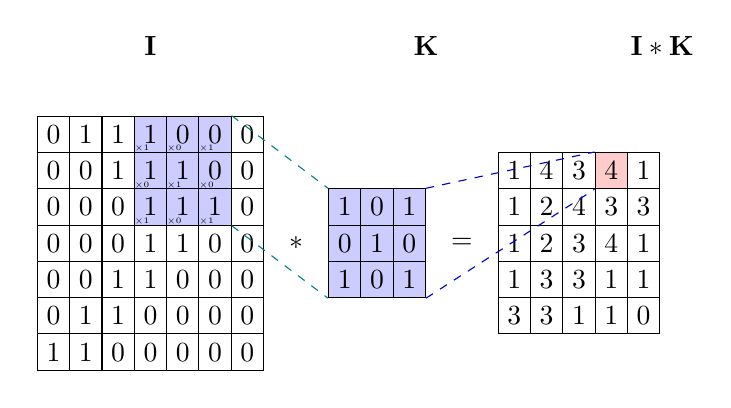
\begin{tikzpicture}[
  2d-arr/.style={matrix of nodes, row sep=-\pgflinewidth, column sep=-\pgflinewidth, nodes={draw}}
]

\matrix (mtr) [2d-arr] {
0 & 1 & 1 & |[fill=blue!20]| 1 & |[fill=blue!20]| 0 & |[fill=blue!20]| 0 & 0\\
0 & 0 & 1 & |[fill=blue!20]| 1 & |[fill=blue!20]| 1 & |[fill=blue!20]| 0 & 0\\
0 & 0 & 0 & |[fill=blue!20]| 1 & |[fill=blue!20]| 1 & |[fill=blue!20]| 1 & 0\\
0 & 0 & 0 & 1 & 1 & 0 & 0\\
0 & 0 & 1 & 1 & 0 & 0 & 0\\
0 & 1 & 1 & 0 & 0 & 0 & 0\\
1 & 1 & 0 & 0 & 0 & 0 & 0\\
};

\node at (0,2.5) {$\mathbf I$};

\node[right=0.2em of mtr] (str) {$*$};

\matrix (K) [2d-arr, right=0.2em of str, nodes={draw, fill=blue!20}] {
  1 & 0 & 1 \\
  0 & 1 & 0 \\
  1 & 0 & 1 \\
};
\node at (3.5,2.5) {$\mathbf K$};

\node[right=0.2em of K] (eq) {$=$};


\matrix (ret) [2d-arr, right=0.2em of eq] {
1 & 4 & 3 & |[fill=red!20]| 4 & 1\\
1 & 2 & 4 & 3 & 3\\
1 & 2 & 3 & 4 & 1\\
1 & 3 & 3 & 1 & 1\\
3 & 3 & 1 & 1 & 0\\
};
\node at (6.5,2.5) {$\mathbf{I * K}$};

\draw[dashed, teal] (mtr-1-6.north east) -- (K-1-1.north west);
\draw[dashed, teal] (mtr-3-6.south east) -- (K-3-1.south west);

\draw[dashed, blue!80!black] (K-1-3.north east) -- (ret-1-4.north west);
\draw[dashed, blue!80!black] (K-3-3.south east) -- (ret-1-4.south west);

\foreach \i in {1,2,3} {
    \foreach \j in {4,5,6} {
        \node[font=\tiny, scale=0.6, shift={(-1.2ex,-2ex)}] at (mtr-\i-\j) {$\times \pgfmathparse{int(mod(\i+\j,2))}\pgfmathresult$};
      }
  }
\end{tikzpicture}
\label{fig:conv2d-example}
\caption{Visualization of 2D convolution being done for 7x7 input with 3x3 kernel. Adapted from~\cite{riebesell_tikz_2020}.}
\end{figure}

Convolutional neural networks are a type of neural networks that heavily utilize convolution operations. Convolution is used to extract features from data, and is defined as
\begin{align}
(f \ast g)(t) = \int_{-\infty}^{\infty}f(t-x)g(t)dx,
\end{align}
where $f$ and $g$ are functions to be convolved. For computer science the discrete convolution is often more interesting
\begin{align}
(f \ast g)(i) = \sum_{m}f(i-m)g(m).
\end{align}
For DNNs we often think about convolution in terms of inputs($f$) and kernels($g$), where input is the useful data we want to extract features from and kernels are the specifically selected values that can extract the wanted features from data.

When working with images, for example in a neural network used for classifying objects in images, we use the two-dimensional expansion of the convolution operation
\begin{align}
Conv2D(i, j) = (K \star I)(i,j) = \sum_{m}\sum_{n}I(i-m,j-n)K(m, n)
\end{align}
where $I$ is the input and $K$ is one kernel, $m$ is the width of the kernel and $n$ is the height.

In high-level deep learning frameworks convolution is often implemented as cross-correlation but still called convolution~\cite{DeepLearningBook,pytorch,tensorflow2015-whitepaper}. This is also what we have done in our implementation
\begin{align}
Conv2D(i,j) = CrossCorrelation(I, K) = (K \star I)(i,j) = \sum_{m}\sum_{n}I(i+m,j+n)K(m, n)
\end{align}
To produce output of one layer one needs to calculate $Conv2D$ for all the positions in the resultant output matrix for all the kernels.

The choice of kernel size determines what kind of features are extracted. Large kernels capture broad features, where small kernels capture finer details.
The specific weights are found during training and that defines which features are to be extracted. Producing good feature maps is thus critical to the performance of the trained CNN.

\subsection{Depthwise Separable Convolution}
As seen in the previous section, convolution is a costly operation to calculate, when the size of inputs and amount of features grows. This is especially difficult for low power hardware that can't parallellize convolution and has to process the operation sequentially.

One common solution for this problem that is often seen in embedded applications, is to use grouped convolution. In grouped convolution we separate the input channels and filters into $G$ groups so that the convolution is only performed among inputs and filters belonging to the same group. The groups essentially behave as completely independent convolution layers in respect to the other groups.  In the end after each input channels has been processed the resulting features get concatenated back into one tensor which has the equal size as the output of same convolution without groups with less calculation.~\cite{howard2017mobilenetsefficientconvolutionalneural, tan_efficientnet_2020}

The computational cost of standard two-dimensional convolution is
\begin{equation}
\text{Cost}_{Conv2D} = K_{x} \cdot K_{y} \cdot I_{x} \cdot I_{y} \cdot C_{in} \cdot C_{out}
\end{equation}
where $K_{x}$, $K_{y}$, $I_{x}$, $I_{y}$ are the dimensions for single kernel and input channels, $C_{in}$ is the number of input features and $C_{out}$ is the number of output features. Whereas the computational complexity of grouped convolution is
\begin{equation}
\text{Cost}_{Grouped} =
  K_{x} \cdot K_{y} \cdot I_{x} \cdot I_{y} \cdot \frac{C_{in} \cdot C_{out}}{G}
\end{equation}
where $G$ is the number of groups. By setting the number of grouped to $G = C_{out}$ we arrive at the special case of grouped convolution called depthwise convolution.

In depthwise convolution each input channel only interacts with its corresponding set of feature kernels giving us a computational complexity which is not dependent on the number of input channels. This effectively removes any interaction across channels, which can limit the amount of features that a CNN can express. To introduce intra-channel interaction to depthwise convolution, we often follow depthwise layer with a pointwise convolution layer. Pointwise convolution is just standard 2D convolution with a filter of size $1 \times 1$, this ensures that output and input have same sized channels. Depthwise followed by pointwise is so common combination that it has its own name, depthwise separable convolution, which has the computational complexity of

\begin{equation}
\text{Cost}_{Separable} =
  K_{x} \cdot K_{y} \cdot I_{x} \cdot I_{y} \cdot  C_{in} + I_{x} \cdot I_{y} \cdot C_{in} \cdot C_{out}
\end{equation}

As shown in~\cite{tan_efficientnet_2020} depthwise separable convolutions can greatly reduce the amount of network parameters and thus reduce the total number of operations during inference without having a noticeable effect on the model accuracy. This makes it a popular layer structure in neural network targeted for mobile devices, like MobileNet~\cite{howard2017mobilenetsefficientconvolutionalneural}.


\subsection{Bias}
In addition to $Conv2d$, bias is another important concept in neural networks. Bias is a constant value applied to output channel of the preceding operation. In CNNs when applied after $Conv2d$ the purpose of bias is to signify the importance of each extracted feature. If bias is small or negative it means that the feature is not important for the particular class it's being applied. If bias is large or positive it means that the feature is important.~\cite{DeepLearningBook}

In mathematic notation bias is defined as such
\begin{align}
y = x^{T}W + b
\end{align}
where if $xA^{T}$ is the non-biased output of a particular channel in layer, $b$ is the bias applied to the whole channel as a constant value. Many DL frameworks consider bias part of the convolution operation and fuse them together into one layer as is done with for example Tensorflow~\cite{tensorflow2015-whitepaper}.

\subsection{Activation functions}
The combination of convolution and bias form one example of an affine transformation, a linear transformation between two space.
To enable neural networks to recognize non-linear features, we need to introduce non-linear operations between the linear affine transformations. Traditionally we used sigmoid or tanh functions, which are defined as

\begin{align}
\sigma(x) = \frac{1}{1+e^{-x}}
\end{align}
and,
\begin{align}
tanh(x) = \frac{e^{x}-e^{-x}}{e^{x}-e^{-x}},
\end{align}
to introduce non-linearity. Both functions suffer from the fact that they are expensive to calculate and exhibit the vanishing gradient problem.~\parencite{DeepLearningBook}

Because of these problems DNNs have largely moved to using Rectified linear units (ReLU) for layer activations~\cite{krizhevsky_imagenet_2012}.
ReLU is a simpler operation, moving negative values to zero and doing nothing for positive values, defined as
\begin{align}
ReLU(x) =
\begin{cases}
0, & \text{for} \leq 0 \\
  x, &  \text{otherwise}.
\end{cases}
\end{align}
ReLU is essentially a special case of the clamp operation, show in equation~\ref{eq:clamp}, where the low bound is set to 0, and high bound as the maximum signed value of the given bit width. This is also how some DL frameworks implement ReLU activation~\cite{TVM}.

Figure~\ref{fig:activation-functions} shows how ReLU and sigmoid non-linearly scale values close to $x=0$. The ReLU is always zero when x is less than zero, and x when greater than zero, making its calculation a matter of checking the signed bit for each element. Sigmoid on the other hand has a curved shape, highlighting the fact that it's more expensive to calculate.

\begin{figure}[ht]
\centering
\begin{minipage}[t]{.45\textwidth}
  \centering
  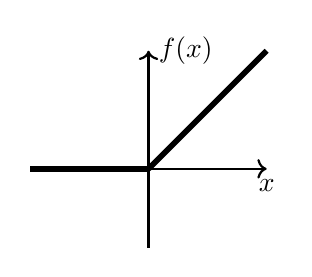
\begin{tikzpicture}
      % Axes
      \draw[thick,->] (-1.5,0) -- (1.5,0) node[anchor=north] {$x$}; % x-axis
      \draw[thick,->] (0,-1) -- (0,1.5) node[anchor=west] {$f(x)$}; % y-axis

      % ReLU function
      \draw[line width=2pt,black] (-1.5, 0) -- (0, 0); % f(x) = 0 for x < 0
      \draw[line width=2pt,black] (0, 0) -- (1.5, 1.5); % f(x) = x for x >= 0
  \end{tikzpicture}
  \captionof{figure}{Rectified linear unit (ReLU)}
\end{minipage}
\begin{minipage}[t]{.45\textwidth}
  \centering
  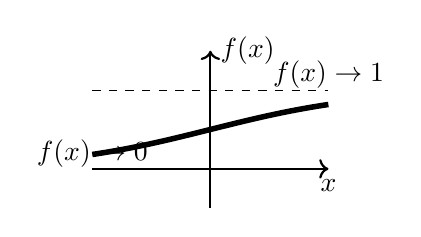
\begin{tikzpicture}
      % Axes
      \draw[thick,->] (-1.5,0) -- (1.5,0) node[anchor=north] {$x$}; % x-axis
      \draw[thick,->] (0,-0.5) -- (0,1.5) node[anchor=west] {$f(x)$}; % y-axis

      % Sigmoid function plot
      \draw[line width=2pt,black,domain=-1.5:1.5,samples=100,smooth] plot (\x, {1/(1 + exp(-\x))});

      % Labels for Sigmoid
      \node at (-1.5, 0.2) {$f(x) \to 0$}; % Description for x -> -∞
      \node at (1.5, 1.2) {$f(x) \to 1$}; % Description for x -> +∞

      % Horizontal lines for asymptotes
      \draw[dashed] (-1.5,1) -- (1.5,1); % y = 1 asymptote
      \draw[dashed] (-1.5,0) -- (1.5,0); % y = 0 asymptote
  \end{tikzpicture}
  \captionof{figure}{Sigmoid activation}
\end{minipage}
\caption{Comparison of ReLU and Sigmoid activation functions}
\label{fig:activation-functions}
\end{figure}


Combining two-dimensional affine transformation and ReLU gives us the basic Conv2D layer found in most image classification network, like Resnet~\parencite{he2015deepresiduallearningimage} and MobileNet~\parencite{howard2017mobilenetsefficientconvolutionalneural}.
And as with bias, some DL frameworks fuse activation function with the convolution operation to form one layer. Giving use the common definition of a single two-dimensional layer in
\begin{align}
ReLU(Conv2D(I, K) + \hat{b}),
\label{eq:conv2d}
\end{align}
where $I$ and $K$ are the respective input and weight tensors of the layer,  $\hat{b}$ is the vector containing channelwise bias values and $ReLU$ function for the hidden activation of the layer.

\section{Layer graphs}
As mentioned before, DNNs are neural networks with one or more hidden layers. Generally the amount of layers correlates to better prediction results, due to the increasing amount learnable parameters being able to capture more complex features.

The relationships between layers can be presented as graphs, where nodes are layers or fused layers and paths are the data flow directions. Figure~\ref{fig:conv2d-layer} displays the equation~\ref{eq:conv2d} as a simple graph were data flow is always from one layers output to next layers input.

\begin{figure}[ht]
\centering
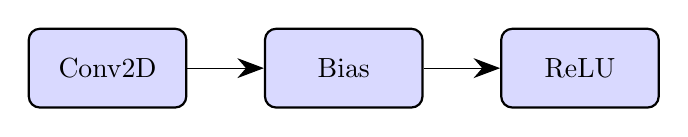
\begin{tikzpicture}
  \node[draw, thick, rectangle, rounded corners, minimum width=2cm, minimum height=1cm, fill=blue!15] (A) at (0,0) {Conv2D};
  \node[draw, thick, rectangle, rounded corners, minimum width=2cm, minimum height=1cm, fill=blue!15] (B) at (3,0) {Bias};
  \node[draw, thick, rectangle, rounded corners, minimum width=2cm, minimum height=1cm, fill=blue!15] (C) at (6,0) {ReLU};

  \path [-{Stealth[scale=2]}] (A) edge node[above] {} (B);
  \path [-{Stealth[scale=2]}] (B) edge node[above] {} (C);
\end{tikzpicture}
\caption{Feed forward relationship between Conv2d, bias and ReLU layers.}
\label{fig:conv2d-layer}
\end{figure}
For clarity this combination of 2D convolution, bias and ReLU is usually fused into single layer node. Different neural network frameworks use slightly different terminology relating to the meaning of operation, layer and fused layer. For example Tensorflow~\parencite{tensorflow2015-whitepaper}, a popular framework for training, considers Conv2D, bias and ReLU separate layers and the combination of a fused layer, whereas in Pytorch~\cite{pytorch} the combination of Conv2D, bias and ReLU is considered one layer. For the purposes of this work, we use Tensorflow naming scheme.

\begin{figure}
\centering
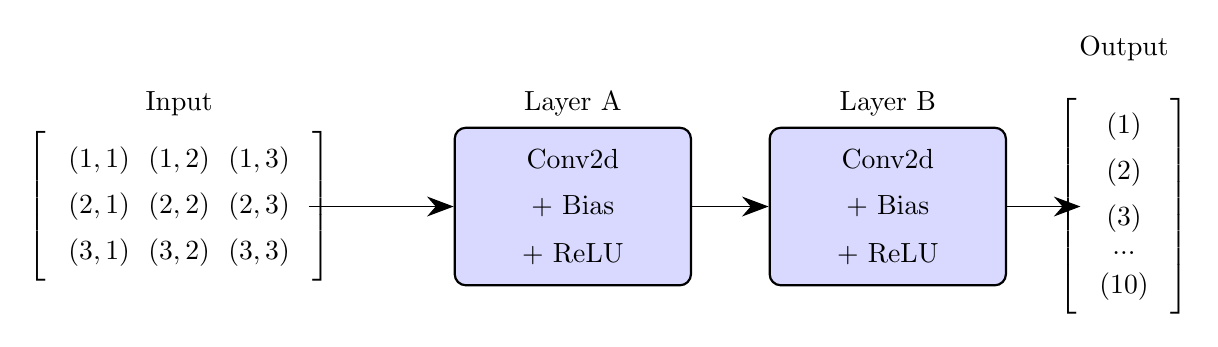
\begin{tikzpicture}
  \node at (-3, 1.3) {Input};
  \matrix [matrix of math nodes, left delimiter={[}, right delimiter={]}, % for the rectangle border
            ampersand replacement=\&] % see explanation
    (mm)
    at(-3, 0)
    {
        \node {(1,1)}; \& \node {(1,2)}; \& \node {(1,3)};\\
        \node {(2,1)}; \& \node {(2,2)}; \& \node {(2,3)};\\
        \node {(3,1)}; \& \node {(3,2)}; \& \node {(3,3)};\\
    };

  % Box A (Layer 1) with sub-nodes Conv2d, Bias, ReLU
  \node[draw, thick, rectangle, rounded corners, minimum width=3cm, minimum height=2cm, fill=blue!15] (A) at (2,0) {};
  \node at (2,1.3) {Layer A}; % Title for Layer 1
  \node at (2,0.6) {Conv2d};
  \node at (2,0) {+ Bias};
  \node at (2,-0.6) {+ ReLU};

  % Box B (Layer 2) with sub-nodes Conv2d, Bias, ReLU
  \node[draw, thick, rectangle, rounded corners, minimum width=3cm, minimum height=2cm, fill=blue!15] (B) at (6,0) {};
  \node at (6,1.3) {Layer B}; % Title for Layer 2
  \node at (6,0.6) {Conv2d};
  \node at (6,0) {+ Bias};
  \node at (6,-0.6) {+ ReLU};

  \node at (9, 2) {Output};
  \matrix [matrix of math nodes, left delimiter={[}, right delimiter={]}, % for the rectangle border
            ampersand replacement=\&] % see explanation
    (out)
    at(9, 0)
    {
        \node {(1)}; \\
        \node {(2)}; \\
        \node {(3)}; \\
        \node {...}; \\
        \node {(10)}; \\
    };

  % Arrow from A to B
  \path [-{Stealth[scale=2]}] (mm) edge node[above] {} (A);
  \path [-{Stealth[scale=2]}] (A) edge node[above] {} (B);
  \path [-{Stealth[scale=2]}] (B) edge node[above] {} (out);
\end{tikzpicture}
\caption{Simple feed forward network with two Conv2D with bias and ReLU activation layers.}
\label{fig:network-simple}
\end{figure}


The simplest kind of relation is a feedforward relationship where the output of layer A is the input of layer B as shown in the figure~\ref{fig:network-simple}. In a simple feedforward connection one instance of a layer output is always exactly input for one layer, without recursion or branching.

Connection can also branch, and the same layer output can be used as input for multiple nodes. Resnet~\cite{he2015deepresiduallearningimage} heavily utilizes what are called residual connections. With residual connection an input of a layer is used in multiple parts of a feed forward network. Figure~\ref{fig:network-residual} shows an example of a residual connection, where input of layer A is used again after concatenation as part of input for layer C.

% In recursive networks an output of a layer can be an input to a layer preceding it, or it's input during the next pass. This kind of structure shown in figure~\ref{fig:recurrent-network} is able to encode time series information, which is heavily used in audio processing and language modeling tasks.

\begin{figure}
\centering
  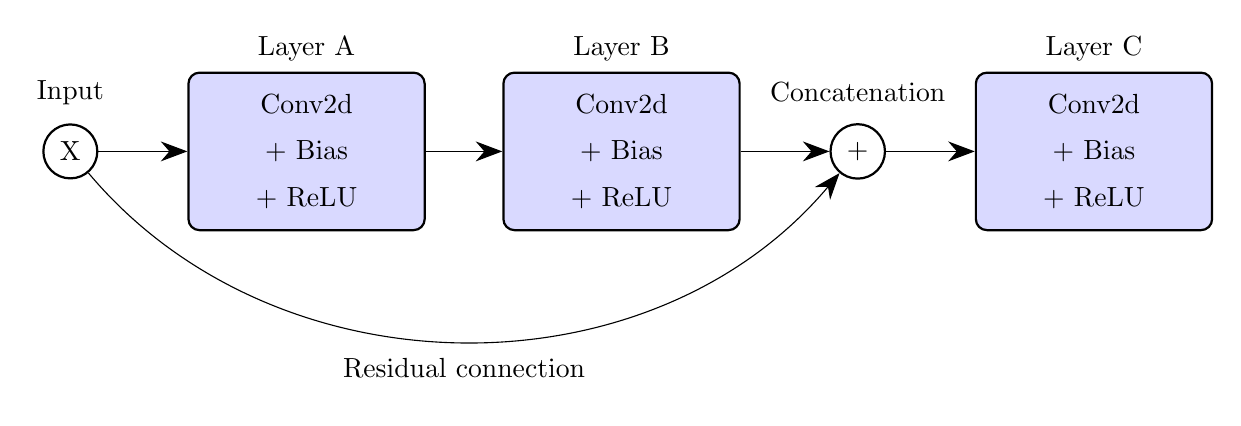
\begin{tikzpicture}
      % Box A (Layer 1) with sub-nodes Conv2d, Bias, ReLU
      \node[draw, thick, rectangle, rounded corners, minimum width=3cm, minimum height=2cm, fill=blue!15] (A) at (0,0) {};
      \node at (0,1.3) {Layer A}; % Title for Layer A
      \node at (0,0.6) {Conv2d};
      \node at (0,0) {+ Bias};
      \node at (0,-0.6) {+ ReLU};

      % Box B (Layer 2) with sub-nodes Conv2d, Bias
      \node[draw, thick, rectangle, rounded corners, minimum width=3cm, minimum height=2cm, fill=blue!15] (B) at (4,0) {};
      \node at (4,1.3) {Layer B}; % Title for Layer B
      \node at (4,0.6) {Conv2d};
      \node at (4,0) {+ Bias};
      \node at (4,-0.6) {+ ReLU};

      % Residual Connection (A to B addition node)
      \node[circle, draw, thick, minimum size=0.6cm] (input) at (-3,0) {X};
      \node[circle, draw, thick, minimum size=0.6cm] (add) at (7,0) {+};
      \node (name1) at (7,0.75) {Concatenation};
      \node (name2) at (2,-2.75) {Residual connection};
      \node (name3) at (-3,0.75) {Input};

      % Arrows from A to B and from B to addition
      %
      \path [-{Stealth[scale=2]}] (input) edge node[above] {} (A);
      \path [-{Stealth[scale=2]}] (A) edge node[above] {} (B);
      \path [-{Stealth[scale=2]}] (B) edge node[above] {} (add);

      % Direct residual connection from A to addition node
      \path [-{Stealth[scale=2]}] (A.east) -- ++(2.5,0) -- (add.west);
      \path [-{Stealth[scale=2]}] (input) edge[bend right=50] node [left] {} (add);

      % Box B (Layer 2) with sub-nodes Conv2d, Bias
      \node[draw, thick, rectangle, rounded corners, minimum width=3cm, minimum height=2cm, fill=blue!15] (C) at (10,0) {};
      \node at (10,1.3) {Layer C}; % Title for Layer B
      \node at (10,0.6) {Conv2d};
      \node at (10,0) {+ Bias};
      \node at (10,-0.6) {+ ReLU};


      \path [-{Stealth[scale=2]}] (add) edge node[above] {} (C);
  \end{tikzpicture}
\caption{Residual feed forward network with fused layers.}
\label{fig:network-residual}
\end{figure}

% \begin{figure}
% \centering
%   \begin{tikzpicture}
%       % Box A (Layer 1) with sub-nodes Conv2d, Bias, ReLU
%       \node[draw, thick, rectangle, rounded corners, minimum width=3cm, minimum height=2cm, fill=blue!15] (A) at (0,0) {};
%       \node at (0,1.3) {Layer A}; % Title for Layer A
%       \node at (0,0.6) {Conv2d};
%       \node at (0,0) {+ Bias};
%       \node at (0,-0.6) {+ ReLU};

%       % Box B (Layer 2) with sub-nodes Conv2d, Bias
%       \node[draw, thick, rectangle, rounded corners, minimum width=3cm, minimum height=2cm, fill=blue!15] (B) at (4,0) {};
%       \node at (4,1.3) {Layer B}; % Title for Layer B
%       \node at (4,0.6) {Conv2d};
%       \node at (4,0) {+ Bias};
%       \node at (4,-0.6) {+ ReLU};

%       % Residual Connection (A to B addition node)
%       \node[circle, draw, thick, minimum size=0.6cm] (input) at (-3,0) {+};
%       \node[circle, draw, thick, minimum size=0.3cm, fill=black] (hidden) at (7,0) {};
%       \node (name2) at (2,2.75) {Recursive connection};
%       \node (name3) at (-3,-0.75) {Addition};

%       % Arrows from A to B and from B to addition
%       %
%       \path [-{Stealth[scale=2]}] (input) edge node[above] {} (A);
%       \path [-{Stealth[scale=2]}] (A) edge node[above] {} (B);
%       \path [-{Stealth[scale=2]}] (B) edge node[above] {} (C);

%       % Direct residual connection from A to addition node
%       \path [-{Stealth[scale=2]}] (A.east) -- ++(2.5,0) -- (add.west);
%       \path [-{Stealth[scale=2]}] (hidden) edge[bend right=50] node [left] {} (input);

%       % Box B (Layer 2) with sub-nodes Conv2d, Bias
%       \node[draw, thick, rectangle, rounded corners, minimum width=3cm, minimum height=2cm, fill=blue!15] (C) at (10,0) {};
%       \node at (10,1.3) {Layer C}; % Title for Layer B
%       \node at (10,0.6) {Conv2d};
%       \node at (10,0) {+ Bias};
%       \node at (10,-0.6) {+ ReLU};


%       \path [-{Stealth[scale=2]}] (add) edge node[above] {} (C);
%   \end{tikzpicture}
% \caption{Recurrent neural network}
% \label{fig:recurrent-network}
% \end{figure}


\section{Neural Model Training}
To perform a given task all neural networks need to be trained. With training the network parameters (weights and biases) are tuned in such a way that the network approximates a function performant in the task. This same concept applies to most model based ML-methods, but with neural network this training is most often done with the backpropagation algorithm. The first step of backpropagation is the forward pass. Forward pass is essentially inference, where the network is given inputs from a known set of inputs with associated ground truth labels for which the network performs predictions. The predictions are then compared with the ground truth with a loss function to calculate current network error. The choice of loss function is critical and poor choice can heavily effect the models potential to discover suitable parameters. Some common loss functions are mean squared error, cross entropy loss and L1 loss.

After forward pass comes the backwards pass, where the parameters of the network are adjusted to minimize the loss function for the given inputs. The tuning is done layer by layer starting from the output layer and working towards the input layer, hence the name backpropagation. To tune the parameters in a way that maximally improves the prediction results, we need to minimize the value of the loss function. To accomplish this we calculate the gradient decent of the network. Essentially gradient descent describe derivative of the n-dimensional space housing the function approximation of the network. Each parameter introduces its own dimension and thus adding a parameter to the derivative.

\begin{equation}
g_{K} = \nabla L (\hat{y}, z_{K}) = \frac{\partial L}{\partial a_{K}} \cdot \frac{\partial a_{K}}{\partial z_{K}},
\end{equation}
where $g$ is the gradient of the last layer's activation in relation to the expected activation as signified by $K$, $L$ is the loss function, $\hat{y}$ is the ground truth or expected prediction, $a_{K}$ is the activation of the output layer or the prediction and $z_{K}$ is the input of the layer.
To find the gradient for the next layer we apply the same chain rule, since we know that the activation of the last layer is dependent on the activation of the previous layer
\begin{align}
g_{K-1}& = \nabla L(\hat{y}, z_{k-1}) = g_{K} \cdot \nabla L(z_{K}, z_{K-1}) \\
& = \frac{\partial L}{\partial a_{K}} \cdot \frac{\partial a_{K}}{\partial z_{K}} \cdot \frac{\partial z_{K}}{\partial a_{K-1}} \cdot \frac{\partial a_{K-1}}{\partial z_{K-1}}.
\end{align}
This same chain rule is applied for the whole graph to produce the complete gradient of the network with final activation in relation to the input $x$
\begin{align}
\nabla L(\hat{y}, x).
\end{align}
Since it's known that the activation of a layer is the affine transformation we know that
\begin{align}
z_{K} = a_{K-1}W_{K} + b_{K} \Rightarrow \frac{\partial L}{\partial W_{K}} = \frac{\partial L}{\partial z_{K}} \cdot a_{K-1}
\end{align}
where $W_{K}$ is the vector of weights for layer $K$.
To tune the weights of a particular layer we need to define an additional term, a learning rate $\eta$ which describe the amount of movement towards the minimum value of the loss function. We can then use the following equation to calculate new weights for all the layers
\begin{equation}
W_{k} = W_{K} - \eta \frac{\partial L}{\partial W_{K}}.
\end{equation}

Biases are also updated with a similar equation
\begin{equation}
b_{k} = b_{K} - \eta \frac{\partial L}{\partial b_{K}}.
\end{equation}


Model training is computationally expensive process and in the case of some of the largest models can take months to train. For this reason it's common to have separate hardware for training and for inference. Training is generally done on GPUs or NNAs with some high-level training network. Whereas inference can be done on different kinds of hardware configurations from server farms to microcontrollers, since the inference is less computationally expensive.

Most training frameworks use 32-bit floating point values to represent rational numbers.~\cite{pytorch}\cite{tensorflow2015-whitepaper}. This allows for the best accuracy in the training. After training the weights and biases can be moved to the target device for inference. Even in the cases where the target model is to be quantized, the network is first trained with high accuracy floating points and quantized afterwards, to represent the rational values with integers to ensure high model accuracy.

\section{Quantization}
When training DNN models with high-level tools like Pytorch, models are built to use floating point values. In recent years quantization has become a well proven optimization technique for improving inference throughput, and reducing the size of models~\cite{wu_integer_2020}. Often there are significant performance gains available by reducing the granularity of the parameters without a major loss in model accuracy as shown~\cite{krishnamoorthi_quantizing_2018,draghici_capabilities_2002}. Standard floating point value has a width of 32-bits, whereas INT8 which is a common integer type in DNNs has just the 8 bits. Thus, when less granularity is acceptable similarly performing integer based accelerator can do 4 times the calculations when compared to a floating point accelerator.
Some models reduce that amount of granularity even more and have layers using 4-bit or 2-bit integers. With 2-bit integers one can do 16-times as many calculations as with floating points, if we suppose hardware that has the same throughput for floating points and integers, with the ability to utilize SIMD instructions. Though, on real hardware integers are almost always faster to calculate than floating points, skewing the performance benefit even more towards quantized integers.

It's also possible to have only parts of the model quantized. For these cases it might be necessary to have additional conversion layers to go from floating point inputs to integers and backwards. This can be useful for the cases where the target platform is only able to accelerate quantized layers, but the developer want's to use well proven subnetwork to ensure accuracy while the rest of the network is hardware accelerated to improve performance.

There are multiple approaches to performing post training quantization, but it essentially always involves representing particular floating point range of a values in layer inputs or outputs with integers fixed to a certain zero point. Zero point encodes the integer value that represents the original domain's value zero in the new domain. Tensorflow uses the affine quantization to quantize the floating point parameters to integers
\begin{equation}
x_{Q} = clamp(0, 255, round(\frac{x_{float}}{\Delta}) + z)
\end{equation}
where $x_{float}$ is the original parameter values, $x_{Q}$ is the quantized parameter value, $z$ is the zero point and $\Delta$ is the scaling factor discovered during quantization.
The clamp operation limits the input to a given range as such
\begin{align}
  \label{eq:clamp}
clamp(a, b, x) =
  \begin{cases}
    a, & \text{for} \; x \leq a  \\
                x, & \text{for} \; a < x < b  \\
                b, & \text{for} \; x \geq b
  \end{cases}.
\end{align}
To convert quantized parameters back to the original parameter values affine quantization uses the following operation
\begin{equation}
x_{float} = (x_{Q}-z)\Delta.
\end{equation}
This back conversion has no need for the clamping operation or rounding, since the floating point range is larger than the 8-bit integer range.

Another choice for quantization is the uniform symmetric which is similar to the affine quantization, but the zero point is always set as 0. This ensures that the negative and positive sides are equal, which is desired of signed integer based accelerators. The equation for quantizing a parameter with the uniform symmetric quantization is as follows
\begin{equation}
x_{Q} = clamp(-128, 127, round(\frac{x_{float}}{\Delta})).
\end{equation}
From the equation we can see that when compared to the affine quantization the zero point term has been removed and the range has been shifted by $-128$. Converting back to the original parameter is as simple as applying the scaling factor
\begin{equation}
x_{float} = x_{Q}\Delta.
\end{equation}
Some integer accelerators might support performing the quatizations in hardware, but generally it's done in software.

\section{Validation and DNN inference evaluation metrics}
\label{sec:metrics}
Model validation is a practice of evaluating the quality of predictions of a neural network. Validation can be done during model training, as well as after training has finished. The purpose of training validation is to detect overfitting, by testing the so far trained model between training loops with data it has not been trained on. The idea is to simulate inference, so that it performs equally well for unseen data as it does with training data.

Post training validation ensures that the trained model still performs in a new platform or environment. For example after a model has been trained on a high-level framework and moved on to a different run time on an another platform, it should be validated to confirm that the new stack works as expected. Different runtime have different implementations of operation and thus the conversion between models, might need additional work from the developer to ensure compatibility.

To evaluate the accuracy of a neural network we measure the amount of correct predictions relative to incorrect predictions. The suitable metric depends on the used codomain's dimensionality and the problem definition. A metric suitable for 100-class classifier might not suit binary classifier.

A single prediction from a binary classifier can have four possible results. Prediction is true positive (TP) when ground truth is positive and the classifier correctly predicted it to be positive. Prediction is true negative (TN) when the ground truth class is negative and the classifier predicts it as negative. False positive (FP) and false negative (FN) predictions happen when the classifier fails to correctly classify the input.

Different problem definitions need to be evaluated with different measures to account for the differing balances between classes. The most common measures are Accuracy, Recall--sometimes called true positive rate (TPR)--and Precision, which are defined as such

\begin{equation}
  \label{eq:accuracy}
\text{Accuracy} =  \frac{\text{TP} + \text{TN}}{\text{TP} + \text{TN} + \text{FP} + \text{FN}}
\end{equation}
\begin{equation}
  \label{eq:recall}
\text{Recall} = TPR = \frac{\text{TP}}{\text{TP} + \text{FN}}
\end{equation}
\begin{equation}
  \label{eq:precision}
\text{Precision} =  \frac{\text{TP}}{\text{TP} + \text{FP}}.
\end{equation}

In addition to these measures there is false positive rate which is the same as Recall, but it measures the relative amount of false positive classification,
\begin{equation}
\text{FPR} = \frac{\text{FP}}{\text{FP} + \text{TN}}.
\end{equation}

To highlight the need for these different metrics let's say we have a binary classifier to validate on a dataset that is extremely one-sided, where $999/1000$ entries are false, and the rest is true. We could make a simple model that always predicts a false. This would give us an accuracy of $99.9\%$, while being totally unable to distinguish between the classes, while the rest of the measures reflect the nature of the model more accurate manner with a value of $0$.~\cite{DeepLearningBook}

\subsection{Top-1}
Top-1 is the most straightforward evaluation metric for multi-class classifiers. In top-1 we simply take the highest classified class and compare that to ground truth. If the predicted class is the same as the ground truth the predictions is counted as correct. This is repeated for all inputs in the validation set, and the final accuracy is determined by the relation of correct predictions to the total number of predictions done.
\begin{equation}
\text{Top-1 Accuracy} = \frac{1}{N} \sum_{i=1}^{N} \delta(\hat{y}_i, \text{argmax}(f(x_i)))
\end{equation}
where $N$ is the total number of inputs in the evaluation, $\delta$ is the Kronecker delta function, $\hat{y}$ is the correct classification of the input, $x_i$ is the input to the classifier and $f()$ is the classifier.

\subsection{AUC}
Area under the curve (AUC) is a metric for evaluating binary classifiers. It compares the relative amount true positive predictions to false positive predictions.
The main benefit of AUC over simple accuracy is that it balances uneven datasets. For binary anomaly detection it's common that the amount of non-anomalous samples is magnitude larger than the amount of anomalous samples.
Most ML libraries approximate the AUC with a discrete AUC using the Trapezoidal Rule~\cite{pytorch}
\begin{align}
\text{AUC} & = \int_{\text{FPR}=0}^{\text{FPR}=1} \text{TPR}(\text{FPR}) \, d(\text{FPR}) \\
& \approx \sum_{i=1}^{n-1} \frac{(\text{FPR}_{i+1} - \text{FPR}_i) \cdot (\text{TPR}_{i+1} + \text{TPR}_i)}{2},
\end{align}
where TPR is the true positive rate, the relative amount of correct positive predictions from all the positive inputs, and FPR is the false positive rate, relative amount of false positive predictions to all negative inputs.

\section{System-on-chip}
The limited growth in single-core performance due to limitations of Dennard scaling~\cite{esmaeilzadeh_dark_2011}, has shifted the focus of CPU designers towards homogeneous multicore architectures.
And the need to overcome Moore's law has made chipmakers move even further towards heterogeneous architectures. Heterogeneous architectures consist of conventional von Neumann CPUs and unconventional computing elements working together to perform calculations. Unconventional computing elements, might include GPGPUs, FPGAs and custom logic units.~\cite{chung_single-chip_2010}

System-on-chips (SoCs) are a form of heterogeneous computing, where multiple different computing elements and electronic systems are integrated into one circuit.~\cite{Greaves2021}
SoCs generally include CPUs, memories, IO interfaces and specialized accelerators, but conceptually there is no set definition on what SoC needs to include.
This essentially produces a single functional entity that can easily integrated into multitude of different general processing workloads.

What separates SoCs from other heterogeneous architectures is its level of integration between computing elements. Interconnects that connect the chips computing elements can be run on very high bitrates, greatly reducing latency. Unified memory architectures and DMAs enable different components to use the same data without needing to rely on the main computing units for access, improving the system's coherency. The single chip design of SoCs give them a noticeable advantage in terms of physical size and energy consumption, when compared to traditional heterogeneous architectures. This has made SoC a popular option for mobile and edge devices, where the physical size and the decreased energy consumption has significantly been able to improve performance.\cite{di_natale_moving_2010}

In recent times SoC have also begun being seen more in consumer laptops, effectively handling desktop workloads as is the case with the Apple M-series of chips~\cite{apple_m1} and Qualcomm's Snapdragon Elite X series of  chips~\cite{snapdragon_x_elite}.



\section{Deep Learning Accelerators}
\label{sec:dlas}
Deep Learning Accelerators (DLAs) or sometimes called Neural Processing Units (NPUs) are hardware accelerators, that accelerate common neural network operations. In many networks, this means accelerating convolution and dense layers by parallellizing the calculation of output elements.

Due to the size of DNNs an accelerator cannot usually fit the whole model in to its memory. This necessitates a need for off-chip memory to store the model, which the accelerator accesses for new data between layers. The consecutive nature of most DNN models also makes it impossible to have a pipelined execution of layers, next layer computation generally cannot begin before the previous is finished. For this reason DLAs usually feature just one central computing element.

In desktop applications and data center workloads neural networks have been accelerated with GPUs, due to their ability to perform linear-algebra operations like matrix multiplication with high amount of parallellity. To improve power efficiency, it's becoming more common for mobile devices to have dedicated DLAs in addition to GPUs. Companies such as Apple and Qualcomm now include multiple mobile DLA's in their SoCs to run applications like face recognition on phones using their chips.

In addition to SoC Hub's Headsail-DLA other organization have developed their own ASIC based accelerator's for DL workloads.
DianNao is one of the first ASIC based accelerators targeting convolutional deep neural networks~\cite{chen_diannao_2014}. It's based on a pipelined NFU, where the multiply and accumulation operations are implemented as a pipeline alongside bias and sigmoid activations. This is unlike more modern designs where the main computational element is a computational array.

Eyeriss~\cite{chen_eyeriss_2017} is an early example of a MAC array based DLA for accelerating convolution networks, focused on high energy efficiency and performance, by minimizing the amount of data transfers. Eyeriss implements convolution 2d operation with bias and ReLU, and it uses 16-bit floating points. Convolutions are executed in a 12 x 14 PE-array, where each PE performs the multiply-accumulate operation for one input feature element at a time. Eyeriss loads current layers parameters from the off-chip dram into it's 108KB global buffer, from which the operation parameter are scattered for the PE-array. PEs heavily utilize scratch pads to improve data access times, by enabling data reuse of the kernels.

\chapter{Methodology}
This section goes over the technologies used to complete this project in detail. First we discuss the hardware used in the SoC Hub's Headsail SoC and the parts affecting the decisions made in the software design in detail. After this we present the used software stack necessary to run neural networks on the described hardware. We will also discuss the virtual prototype on which the majority of the software development took place on, and how it differs from the hardware. Finally we will describe the MLPerf Tiny benchmark, which is our use-case for the DLA.
\label{ch:methodology}

\section{Headsail}
Headsail is the third SoC build by the SoC Hub research group~\parencite{Ballast}. Headsail has two RISCV CPUs, one 32-bit meant for booting up the system called SysCtrl and one 64-bit 4-core CPU called HPC, meant for running the actual applications, based on the CVA6~\cite{zaruba2019costCVA6}.
Headsail includes a wide variety of different peripherals, one of which is a custom-built the Deep Learning accelerator.
For I/O headsail has UART, SPI and I2C connectivity.
In addition to CPU bootrams, Headsail features 256 megabytes of SDRAM and 128 kilobytes of shared SRAM. This abundance of memory gives application space developers lots of flexibility for their applications. Considering that even small neural networks need megabytes of memory, large memory will be vital for the success of this project.

\subsection{DLA}
Headsail's DLA is a MAC array based accelerator, which provides the following operations: Conv2D, Bias, ReLU. The operations are implemented as a pipeline, meaning that the order of operations is always the same. During one layer cycle the operations need to be executed in the following order: Conv2d, Bias, ReLU. This is the most commonly found order in modern neural networks so it suits most use cases. In addition to these operations DLA can perform bit shifting for results of the MAC array and the post-processing pipeline.
Bias and ReLU can be skipped in the case neither of them is needed in the given layer. In this case Conv2D output is used directly and is capped to fit the 8-bit width of the output.
The particular operations are configured from the register interface of the DLA.
DLA has a simple 32 bit RISC-V based controller CPU, that can be used to drive the DLA parallel to normal HPC execution, but it's also possible to control the DLA directly from the main CPUs. Which is what we have opted to for this project.

The input and weights are fed to the MAC array from the sixteen 32 kilobytes sized memory banks. The input and weights need to be written into separate banks and the data needs to be continuous and in the case the data doesn't fit into a single bank the neighboring bank needs to be used. The bias values for the post-processing step are fetched from the Headsail's SDRAM and can be located in any arbitrary point of memory.

\section{TVM}
TVM is a machine learning compiler framework by Apache. Among other features TVM includes, multiple runtimes, accelerator backends, optimizers, and a machine learning library for building and training models. The variety of features allows for TVM to be used to implement a complete machine learning workflow, or TVM can be used to implement part of the workflow with other tools.

TVM implements its own graph representation for neural network with its Relay IR graphs, which similarly to other graph representation represents network layers as nodes in a abstract syntax tree.
In the graph, data flow is signified by the directional vertices connecting the nodes, in such a way that the output of the node the data travels from acts as the input for the child node at the end of the vertex. The Relay IR support multitude of different transformations to manipulate the operations performed in the network. This enables developers to write transformation passes to modify certain nodes of patterns of nodes to ensure that the graph is compatible with different hardware configurations.

TVM can be extended to support additional hardware accelerators by implementing a custom code generation module for the target hardware. In principle the developer defines external C symbols that provide the operation implementations which TVM then injects into the Relay IR models. During runtime TVM then calls these external symbols instead of the default operations provided by the TVM Relay library.

It's possible to generate Relay IR models from other graph formats with TVM. For example common formats like Tensorflow, Torch and ONNX~\cite{onnxruntime} models are officially supported by TVM. This allows developers to build and train their models with tools they might prefer over TVM, and use TVM as a compiler/runtime.

TVM has the ability to take most of the common ML training graphs and convert them to TVM Relay graph. Figure~\ref{fig:tflite-to-tvm} shows the conversion of a quantized Tensorflow Conv2d layer into corresponding relay graph. From the figure we can see that TVM separates nodes into smaller entities, where each node performs one options, instead of the fused approach of Tensorflow. This gives developers more control over which operations to assign for which hardware.
During model compilation TVM is able to optimize the graph and allocate acceleratable nodes to suitable accelerators.~\parencite{TVM}

\begin{figure}
\centering
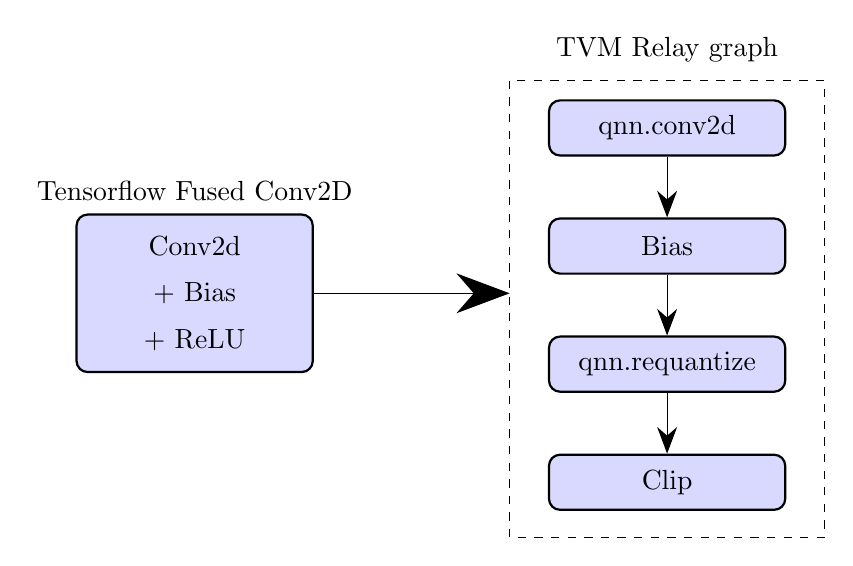
\begin{tikzpicture}
    \node[draw, thick, rectangle, rounded corners, minimum width=3cm, minimum height=2cm, fill=blue!15] (A) at (-3,-2.1) {};
    \node at (-3,-0.8) {Tensorflow Fused Conv2D}; % Title for Layer A
    \node at (-3,-1.5) {Conv2d};
    \node at (-3,-2.1) {+ Bias};
    \node at (-3,-2.7) {+ ReLU};

    % Box for Qnn.conv2d
    \node[draw, thick, rectangle, rounded corners, minimum width=3cm, minimum height=0.7cm, fill=blue!15] (Qnn) at (3,0) {};
    \node at (3,0.0) {qnn.conv2d};

    % Box for Bias
    \node[draw, thick, rectangle, rounded corners, minimum width=3cm, minimum height=0.7cm, fill=blue!15] (Bias) at (3,-1.5) {};
    \node at (3,-1.5) {Bias};

    % Box for Qnn.requantize
    \node[draw, thick, rectangle, rounded corners, minimum width=3cm, minimum height=0.7cm, fill=blue!15] (Requantize) at (3,-3) {};
    \node at (3,-3) {qnn.requantize};

    % Box for Clip
    \node[draw, thick, rectangle, rounded corners, minimum width=3cm, minimum height=0.7cm, fill=blue!15] (Clip) at (3,-4.5) {};
    \node at (3,-4.5) {Clip};

    % Box for outline
    \node at (3,1.0) {TVM Relay graph};
    \draw[dashed] (1, 0.6) rectangle (5, -5.2);

    % Arrows
    \path [-{Stealth[scale=2]}] (Qnn) edge node[above] {} (Bias);
    \path [-{Stealth[scale=2]}] (Bias) edge node[above] {} (Requantize);
    \path [-{Stealth[scale=2]}] (Requantize) edge node[above] {} (Clip);
    \path [-{Stealth[scale=4]}] (A) edge node[left] {} (1, -2.1);
\end{tikzpicture}
\caption{Tensorflow layer to TVM relay graph conversion}
\label{fig:tflite-to-tvm}
\end{figure}

\subsection{Runtimes}
The function of a neural network runtime is to enable other parts of the program to make predictions using the neural network. To do this runtime needs to know when to apply which operation and with which parameters. TVM offers two different runtimes. First is the graph executor runtime. The graph executor takes the graph representing the neural network and traverses it in order to know which operations to execute. The graph executor also needs a separate data structure for the neural network parameters, which the graph has mappings for. During execution the executor fetches the necessary parameters for each operation based on the reference in a given node matching to the parameters.

The other option for a runtime is the Ahead-of-Time runtime (AOT) which takes the same graph and parameters as with graph executor, but instead of dynamically fetching the operations and parameters during execution, the AOT runtime compiles the graph into executable C code or machine code. The AOT then produces a simple API with entry points for input data and execution call, for running predictions in a program. When the program calls for prediction the graph traversing is done by simple calling a next node in the graph as a function, where the execution of a specific operation is defined programmatically, and the necessary parameters are set in place.

The main difference between the runtimes is that graph executor is more dynamic. The executed network and parameters can be redefined during runtime. The AOT is more rigid. All the possible networks need to be embedded directly into the binary of the program. This rigidity comes with simplicity. The API of the AOT is really simple to use, consisting of only the data input and run call. Graph executor, requires more setup from the program, such as parsing the JSON to obtain the graph, and dynamically loading the parameters for each node. For the purposes of this project we settled on using the AOT.

\subsection{Graph Transformations}
To assign calculations for an accelerator the Relay graph of a network needs to be transformed, in such a way that the resulting graph is compatible with the device. In addition to conversion from a different framework to relay, the relay graph needs to be legalized for a specific target and acceleratable patterns needs to be assigned for suitable hardware.

In TVM the first transformation pass is the legalization, where the graph is traversed, and certain parameters are recalculated to fit the target. For example when executing a unsigned 8-bit quantized network most models use a zero point of $-128$ to mimic signed behaviour. If this network is run on an accelerator with support for signed integers, this zero point needs to be changed to 0, since there is no need for the adjustment. If this network is run on an accelerator with support for signed integers, this zero point needs to be changed to 0, since there is no need for the adjustment. This can be done in the legalization pass.

The other transformation pass is the graph annotation. By default, all the operation are assigned to the CPU. With graph annotation certain patterns of nodes can be annotated to be executed with additional accelerators. The patterns are similar to regexes, where a sequence of nodes, for example Conv2D followed by a bias node can be fused together into single composite node.

During code generation with the AOT runtime, TVM traverses the graph and generates code to execute each node. If the node or composite node is annotated to be executed on an accelerator TVM refers to the corresponding code generation backend to produce code for executing the operation. This exposes a way for developers for integrating new accelerators for TVM.

\subsection{BYOC}
``Bring your own codegen'' or BYOC, is one of the possible APIs for integrating new devices into TVM.
With BYOC, developers define target specific relay backend to generate C code for executing the annotated patterns in the model graph.
The backend is created by defining \texttt{CallNode} operators that are called when the backend traverses a network graph during code generation.
These operators extract the needed information of the nodes for use with the target's deep learning API.
Target backend is defined as a C++ module in TVM relay backend and can output either C code or object code when supplied with TVM's LLVM integration.

\begin{figure}
\centering
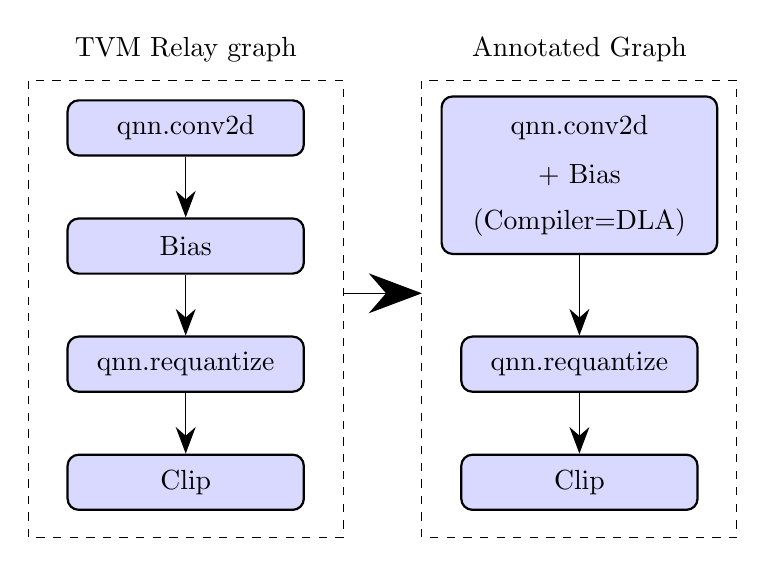
\begin{tikzpicture}
    % Box for Qnn.conv2d
    \node[draw, thick, rectangle, rounded corners, minimum width=3cm, minimum height=0.7cm, fill=blue!15] (Qnn) at (0,0) {};
    \node at (0,0.0) {qnn.conv2d};

    % Box for Bias
    \node[draw, thick, rectangle, rounded corners, minimum width=3cm, minimum height=0.7cm, fill=blue!15] (Bias) at (0,-1.5) {};
    \node at (0,-1.5) {Bias};

    % Box for Qnn.requantize
    \node[draw, thick, rectangle, rounded corners, minimum width=3cm, minimum height=0.7cm, fill=blue!15] (Requantize) at (0,-3) {};
    \node at (0,-3) {qnn.requantize};

    % Box for Clip
    \node[draw, thick, rectangle, rounded corners, minimum width=3cm, minimum height=0.7cm, fill=blue!15] (Clip) at (0,-4.5) {};
    \node at (0,-4.5) {Clip};

    % Box for outline
    \node at (0,1.0) {TVM Relay graph};
    \draw[dashed] (-2, 0.6) rectangle (2, -5.2);

    % Box for composite
    \node[draw, thick, rectangle, rounded corners, minimum width=3.5cm, minimum height=2cm, fill=blue!15] (Composite) at (5,-0.6) {};
    \node at (5,0.0) {qnn.conv2d};
    \node at (5,-0.6) {+ Bias};
    \node at (5,-1.2) {(Compiler=DLA)};

    % Box for Qnn.requantize composite
    \node[draw, thick, rectangle, rounded corners, minimum width=3cm, minimum height=0.7cm, fill=blue!15] (RequantizeComposite) at (5,-3) {};
    \node at (5,-3) {qnn.requantize};

    % Box for Clip composite
    \node[draw, thick, rectangle, rounded corners, minimum width=3cm, minimum height=0.7cm, fill=blue!15] (ClipComposite) at (5,-4.5) {};
    \node at (5,-4.5) {Clip};

    % Box for outline
    \node at (5,1.0) {Annotated Graph};
    \draw[dashed] (3, 0.6) rectangle (7, -5.2);

    % Arrows
    \path [-{Stealth[scale=2]}] (Qnn) edge node[above] {} (Bias);
    \path [-{Stealth[scale=2]}] (Bias) edge node[above] {} (Requantize);
    \path [-{Stealth[scale=2]}] (Requantize) edge node[above] {} (Clip);
    \path [-{Stealth[scale=2]}] (Composite) edge node[above] {} (RequantizeComposite);
    \path [-{Stealth[scale=2]}] (RequantizeComposite) edge node[above] {} (ClipComposite);
    \path [-{Stealth[scale=4]}] (2,-2.1) edge node[left] {} (3, -2.1);
\end{tikzpicture}
\caption{Graph transformation for DLA-vp}
\label{fig:tvm-graph-annotation}
\end{figure}


\subsection{TVM on baremetal}
TVM also provides a tool to run TVM models on bare-metal platforms called microTVM. MicroTVM is only dependent on the C standard library and thus can be used in any bare-metal system that has a working C-toolchain.

MicroTVM works by generating platform independent C-source code from Relay IR-models, which can then be integrated with the microTVM AOT runtime to produce executable binaries to run the network.

The DNN operation implementation are provided by TVM Relay library.
With custom code generation it's also possible to define bare-metal compatible accelerator nodes, which the TVM runtime is able to assign layers for during the C source code generation.~\parencite{TVM}

\subsection{TVM quantization}
TVM implements quantization with its own QNN-dialect~\cite{jain_efficient_2020}. The QNN-dialect separates quantized and non-quantized operations from each other by categorizing the quantized operations under the \texttt{qnn.op} class. QNN operations have additional arguments to indicate scaling factor and zero point for inputs and outputs that are not present in floating point operations.
Where zero points describe the value in the transformed domain that corresponds with the value zero in the origin domain.

In addition to having quantized version of the DL operations the QNN dialect introduces operators for moving data across from non-quantized domain to quantized and back. This is done with the \texttt{qnn.quantize}, \texttt{qnn.dequantize} and \texttt{qnn.requantize} operators. \texttt{qnn.quantize} performs affine quantization to a floating point tensor to produce a corresponding quantized integer tensor, whereas \texttt{qnn.dequantize} reverses the affine quantization. \texttt{qnn.requantize} converts a quantized tensor to another quantized tensor corresponding with a different scale than the original.

TVM enables compatibility of quantized networks with other major DNN frameworks like tensorflow with QNN-dialect aware graph parsing. When model from another framework is parsed into Relay graph, the framework specific quantization operations get converted to QNN nodes. The resulting graph is then passed through canonicalization and legalization passes to produce relay graph that can be annotated for a target.
Canonicalization pass converts the QNN nodes into relay operations. For example \texttt{qnn.Conv2d} gets broken into, dequantization, floating point convolution, bias, requantization to integer values and clipping operations.
In legalization pass the canonicalized relay graph is transformed into relay graph that is compatible with the target hardware. For example this might include rewriting zero points in requantization nodes, or recasting inputs to fit the target device.
After legalization the graph can be annotated and acceleratable patterns can be assigned for the targets.

\section{Renode}
\label{sec:renode}
Renode is a high-level full system emulator, which enables developers to rapidly develop hardware dependent software~\cite{renode}. In essence Renode allows the user to specify exactly which kind of hardware they want to target, down to the implementation of specific peripherals and memory addresses. This streamlines the process of HW/SW integration, since hardware and software can be developed in parallel, which in return reduces the total production time for products.

Renode models a wide variety of different processors and peripherals, but it is also expandable with custom components that are either baked directly into the binary (source code extensions in C\#) or with dynamically loaded Python peripherals. Python peripherals are more limited when compared to the C\# peripherals, since they can't be connected to the clock domain of the system and can only change state when their memory region is accessed. Renode's Python peripherals are also executed in a separate IronPython~\cite{ironpython} container that at this moment, only support modules from Python standard library.

While Renode is an operation accurate emulator, the Python API isn't. When Renode makes a request to the Python API, it counts as one clock cycle even when realistically the Python API's corresponding hardware implementation would take more than one cycle. The consequence of this that we cannot accurately benchmark DLA in Renode. The benefit of the Python API is in rapid development of emulated hardware components.

Renode integrates with the Robot testing framework~\cite{robotframework} to enable automated testing of Renode devices. This makes it possible to use principles of continuous integration and continuous delivery for Renode projects and hardware dependent software.

\section{MLPerf Tiny}
\label{sec:tinyperf}
MLPerf Tiny is a benchmarking suite for benchmarking ML inference in low power targets, like MCUs with Deep Learning Accelerators.~\parencite{tinyperf}
MLPerf Tiny consists of four benchmarks meant to target different use cases shown in table~\ref{tab:tinyperf}.

\begin{table}[ht]
\centering
\caption{Tiny Performance Benchmarks, from~\parencite{tinyperf}}
\begin{adjustbox}{max width=\textwidth}
\begin{tabular}{lccc}
  \toprule
  \textbf{Benchmark} & \textbf{Dataset (Input Size)} & \textbf{Model (TFLite Model Size)} & \textbf{Quality Target (Metric)} \\
  \midrule
  Keyword Spotting & Speech Commands (49x10) & DS-CNN (52.5 KB) & 90\% (Top-1) \\
  Visual Wake Words & VWW Dataset (96x96)  & MobileNetV1 (325 KB) & 80\% (Top-1) \\
  Image Classification & CIFAR10 (32x32) & ResNet (96 KB) & 85\% (Top-1) \\
  Anomaly Detection & ToyADMOS (5x128)  & FC-AutoEncoder (270 KB) & .85 (AUC) \\
  \bottomrule
\end{tabular}
\end{adjustbox}
\label{tab:tinyperf}
\end{table}
Each of the four tasks uses a different model, dataset and problem definition, to ensure testing of wide amount of workloads. Each of the tasks has a minimum quality requirement to be considered acceptable for the benchmark to be officially submitted. For the three multi-class classifiers the used metric is top-1 and for anomaly detection the metric is AUC.

Since MLPerf Tiny aims to suit most kinds of targets, they give the users lot of freedom in the implementation of the models. In the benchmarks the only performance metric is the actual inference times, as long as the quality requirement is fulfilled. This allows for devices with limited IO capabilities a fair comparison against more capable devices. There is no limitation on the model's data type so MLPerf Tiny can be used to compare between signed and unsigned integer accelerators, as well as with FP8 and FP32 accelerators.
In this project we used the pretrained reference models offered by MLPerf for the benchmark, but the specification also allows for training of new models as long as the architecture is preserved.

\subsection{Image Classification}
\label{sec:tinyperf-ic}
The image classification task aims to classify images from the CIFAR-10 dataset~\cite{Cifar10Krizhevsky09learningmultiple}. CIFAR-10 popular dataset that includes 32x32 RGB color images, each belonging to one class. The 10 classes of CIFAR-10 are labeled as, airplane, automobile, bird, cat, deer, dog, frog, horse, ship and truck.

To do this classification MLPerf Tiny uses Resnet~\cite{he2015deepresiduallearningimage}. Resnet is an implementation of ImageNet~\cite{krizhevsky_imagenet_2012}, where between every pair of layers there is a residual connection added from the pair preceding the previous pair.
The backbone architecture introduced in ImageNet uses multiple consecutive layers of 3x3 kernel size 2D convolutions, to which ResNet introduces residual connections.
Resnet architectures vary by the depth of the network, i.e. number of layers. For example Resnet-50 has 50 layers and Resnet-34 has 34. The image classification task uses custom ResNet-9, which lacks the downsampling pooling layers to compensate for the low resolution of CIFAR-10 dataset.

\subsection{Visual Wake Words}
In the Visual Wake Words (VWW) task, the goal is to identify if at least one person is present in an image from the MSCOCO 2014 dataset~\cite{lin_microsoft_2015}.
The training dataset consists of RGB images preprocessed to the size of 96x96 pixels, featuring at least one person. The testing set, which the benchmark uses features images of the same size, but some have people and some do not.

The model chosen for the VWW is MobileNetV1~\cite{howard2017mobilenetsefficientconvolutionalneural}
Backbone of MobileNet consists of 13 depthwise-separable convolution layers, which are followed by a classifier consisting of average pooling layer and a FC-layer. This architecture makes it the largest model in the benchmark both in terms of parameters and the number of layers.

\subsection{Keyword Spotting}
The keyword spotting task is an audio processing task where the goal is to identify spoken keyword from multiple sound sources. Data used dataset is the Speech Commands V2 dataset~\cite{warden_speech_2018}, consists of short clips where one of 30 words possible words are pronounced. From these words ten are used as keywords alongside background noise and rest of the words as unknown, to produce 12 labels. The samples are converted to spectrograms, allowing us to use a proven image classification network for the classification.

MLPerf Tiny uses model called DS-CNN for the KWS task.
DS-CNN is very similar to MobileNet, in that it heavily utilized depthwise convolutional layers for the backbone.~\cite{shaheed_ds-cnn_2022}
Where MobileNet used 13-layers DS-CNN only has four depthwise-separable convolution layers. Which makes it the smallest model in the benchmark, both by the number of layers and parameters.
Similarly to MobileNet, DS-CNN has a average pooling layer followed by a FC-layer for classifier.

\subsection{Anomaly Detection}
The dataset for this task is the DCASE2020 dataset~\cite{koizumi_description_2020}. DCASE2020 consists of sound samples from the following labels: slide rails, fans, pumps, valves, toy-cars, toy-conveyors, from which the AD task only detects anomalies from the toy-cars.

For the model AD task uses a custom FC-AutoEncoder~\cite{tinyperf}.
Originally proposed by~\cite{rumelhart_learning_1987}, AutoEncoder consists of three parts. First is the encoder which encoder the input and downsamples it to latent space. Second part is the latent space which holds the useful high-level features of the input. Last is the decoder which decodes the latent features and upsamples these features back to original dimensionality of the input.~\cite{chen_auto-encoders_2023} The used FC-AutoEncoder model consists of 10 FC-layers with ReLU activations, from which the first 4 make up the encoder, fifth forms the latent space, the four after latent space make up the decoder and last layer performs the classification.

\chapter{Implementation}
\label{ch:implementation}
This section covers the actual implementation of the used software stack in detail and the specific use cases developed on top of the stack. We first discuss the implementation of the SoCs virtual prototype, and some of its issues. We then cover the implementation of the software stack in great detail. Finally, we present the benchmarking approach with the complete software architecture

\section{headsail-vp}
To enable software development for Headsail before the arrival of the ASICs, we modeled the SoC as a Renode virtual platform~\cite{renode}, which we call headsail-vp. With headsail-vp we aimed to replicate the complete memory map of Headsail, with both processors and some of the peripherals.
The aim with the virtual platform was to kick-start software development for the ASIC and to give developers a more streamlined development environment.
We hoped that headsail-vp would enable faster software development, by removing some friction associated to working on the ASIC, as well as giving use the possibility of modifying the design in the case of hardware bugs.
Additionally, this knowledge in developing virtual prototypes of chip could allow us to better define the hardware specs based on the software demonstrators we develop in for the future chips.
Renode's integration with RobotFramework allowed us to set up a CI/CD pipeline with Github actions from the beginning, ensuring the functionality of new features.

\subsection{DLA-vp}

\begin{figure}
\centering
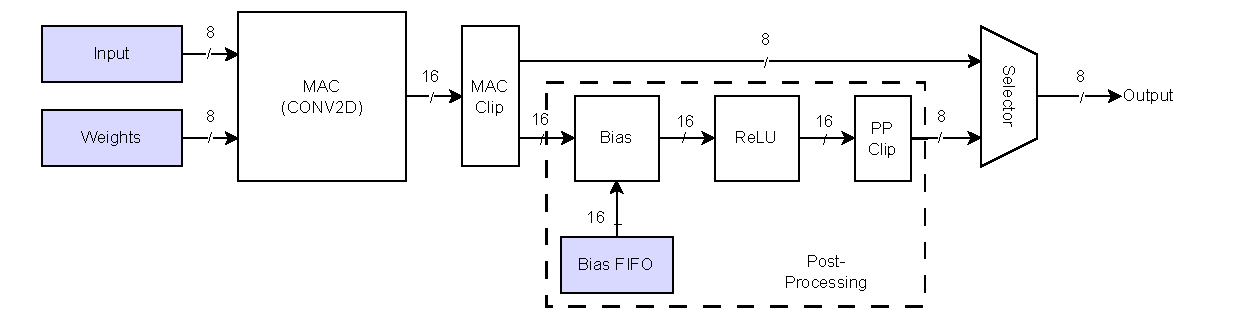
\includegraphics[width=\linewidth]{img/dla-internal.pdf}
\caption{Architecture of accelerated DLA flow in Headsail with TVM runtime and a Pytorch model}
\label{fig:dla_internal}
\end{figure}

Since wanted to develop a use-case for the Headsail DLA with the virtual platform, but because the DLA is a custom ASIC design we had to model it in Renode ourselves. From the two possible options of adding new peripherals to Renode, we chose to use the Python peripheral API. This decision was due to the developer's confidence in writing Python rather than C\#, and the interest in seeing if a peripheral of this size could be successfully implemented with the more limited API.

The DLA-vp supports all the same operations as the ASIC implementation, with identical register interface and same data buffer architecture. This allowed us to develop the driver for the DLA completely on the VP first. After the ASICs where ready we could confirm that the DLA driver was indeed usable on both VP and ASIC. Figure~\ref{fig:dla_internal} shows the high-level structure of the DLA, featuring the input buffer as colored block and the functional blocks in white. This high-level processing pipeline is followed with both the ASIC implementation and in DLA-vp.

DLA-vp implements the register interface as a list of same length. Since numbers in Python can be infinite in length we had to carefully sanitize all the transactions to the registers, so that no accesses over 8-bit values were possible. This same sanitation logic also applied to writing results to the output buffer, since on ASIC all output buffer entries are signed 8-bit values.

Since Renode Python peripherals don't have a clock, the state of the peripheral can only be changed when a CPU reads or writes to an address that is registered for the peripheral. DLA-vp is designed to run a processing loop after each write to its memory region, that checks if the state of DLA-vp is ready for operation execution and if yes, performs the operation per configuration. Read accesses don't change the internal state of the device, so the processing loop isn't executed on them. After executing the processing loop after a write call, the result of the operation can be read on the next clock cycle from the peripheral's memory region.

To verify that the DLA-vp functionally behaved like the hardware implementation of the DLA, we implemented some of the same verification tests done by the hardware team with our software stack. Using the same inputs as the RTL tests with DLA-vp we expect the results to be identical. We implemented the same tests for the low-level driver as well as the high-level driver to ensure that the DLA-vp, as well as the complementing software stack, matches the behaviour of the hardware implementation. This included reimplementing the bugs and design oversights that reduce the accuracy and possibly performance. We integrated these same verification tests to our CI/CD to ensure changes that would break the functional correctness of the DLA would not get merged.

\subsection{Result width limitation}
\begin{figure}
  \centering
  \begin{tikzpicture}[
  2d-arr/.style={matrix of nodes, text centered, row sep=-\pgflinewidth, column sep=-\pgflinewidth, text height=2ex,text width=1.85em, nodes={draw, fill=blue!20}},
  2d-arr-small/.style={matrix of nodes, text centered, row sep=-\pgflinewidth, column sep=-\pgflinewidth, text height=2ex,text width=1em, nodes={draw, fill=blue!20}}
]

    \matrix (B) [2d-arr, right=0.1em of eq, nodes={draw}] {
      -306 & 756 \\
      -74 & -337 \\
    };
    \node at (6.3,1.0) {\textbf{Result}};

    \matrix (C) [2d-arr, right=2.5em of B, nodes={draw}] {
     |[fill=red!20]| -128 & |[fill=red!20]| 127 \\
      -74 & |[fill=red!20]| -128 \\
    };

  \matrix (D) [2d-arr, above=1.5em of C, nodes={draw}] {
     |[fill=red!20]| -5  & |[fill=red!20]| 11 \\
     |[fill=red!20]| -2 & |[fill=red!20]| -6 \\
    };

  \node at (7.9,0.6) {$\text{clip}_0$};
  \node at (7.9,1.7) {$\text{clip}_6$};
  \path [|->] (B) edge node[above] {} (C);
  \path [|->] (B) edge node[above] {} (D);

  \matrix (C2) [2d-arr, right=1.5em of C, nodes={draw}] {
     |[fill=red!20]| -128 & |[fill=red!20]| 127 \\
      -74 & |[fill=red!20]| -128 \\
    };

  \matrix (D2) [2d-arr, right=1.5em of D, nodes={draw}] {
     |[fill=red!20]| -320  & |[fill=red!20]| 704 \\
      |[fill=red!20]|-128 & |[fill=red!20]| -384 \\
    };

  \node at (11,1.0) {$\text{rshift}_N$};
  \path [|->] (C) edge node[above] {} (C2);
  \path [|->] (D) edge node[above] {} (D2);

\matrix (C3) [2d-arr, right=1.5em of C2, nodes={draw}] {
     |[fill=red!20]| 0.58 & |[fill=red!20]| 0.83 \\
      0.0 & |[fill=red!20]|  0.62 \\
    };

  \matrix (D3) [2d-arr, right=1.5em of D2, nodes={draw}] {
     |[fill=red!20]| 0.05  & |[fill=red!20]| 0.07  \\
     |[fill=red!20]| 0.73  & |[fill=red!20]| 0.14 \\
    };

  \node at (14,1.0) {$\text{error}$};
  \path [|->] (C2) edge node[above] {} (C3);
  \path [|->] (D2) edge node[above] {} (D3);

  \matrix (C4) [2d-arr, right=1.5em of C3, nodes={draw}] {
     |[fill=red!20]| 0.51 \\
    };

  \matrix (D4) [2d-arr, right=1.5em of D3, nodes={draw}] {
     |[fill=red!20]| 0.25 \\
    };

  \node at (17,1.0) {$\text{error}_{avg}$};
  \path [|->] (C3) edge node[above] {} (C4);
  \path [|->] (D3) edge node[above] {} (D4);

  \end{tikzpicture}
  \caption{Example of the result reading procedure from DLA with two different clipping values, and their effect on the retrieved values.}
  \label{fig:clip-matrix}
\end{figure}


\label{sec:result-width-problem}
A major limitation of the DLA's design in respect to accelerating abritrary models, is its limited bit width of the output elements. A single element in the output tensor is represented with a signed byte and thus has the value in the range from $-128$ to $127$. This can be seen from the figure~\ref{fig:dla_internal} where the bit-width of data is reduced in half after the MAC clip and PP clip blocks. This inevitably has the consequence that we will lose some accuracy of results when we move data back to the CPU. The amount of inaccuracy depends on the amount of clipping we perform in the clipping step. DLA has the ability to clip any sequence of 8-bits from the 16-bit sequence that is each result tensor element.

Figure~\ref{fig:clip-matrix} shows and example of the clipping behaviour for two different clipping value for two different clipping values. In the figure the Result matrix is some arbitrary convolution result from the MAC array, which gets applied clipping values of $0$ which means that we don't clip the result, giving us the 8 least significant bits as the read result. The second clipping amount is $6$. In the driver we perform right shifting to reverse the effect of the clipping giving as results in the correct magnitude. By taking the difference between the original values and the right shifted values we can get the element-wise and average amounts of error in for both clipping values.

In figure~\ref{fig:clipping} we have repeated this procedure for all nine possible clipping values and plotted the results. From these results we can see that for this particular result the best accuracy is retrieved with clipping amount of 3. For different matrices the optimal clipping value will be something different. Choosing this result poorly can cause complete error of the results as shown with the result of clipping value of 8.
This behaviour is the most significant cause on incompatibility between the DLA and DNNs trained on high-level frameworks, such a Tensorflow lite, and mitigating its effect were a major challenge for this project.

\begin{figure}
  \centering
  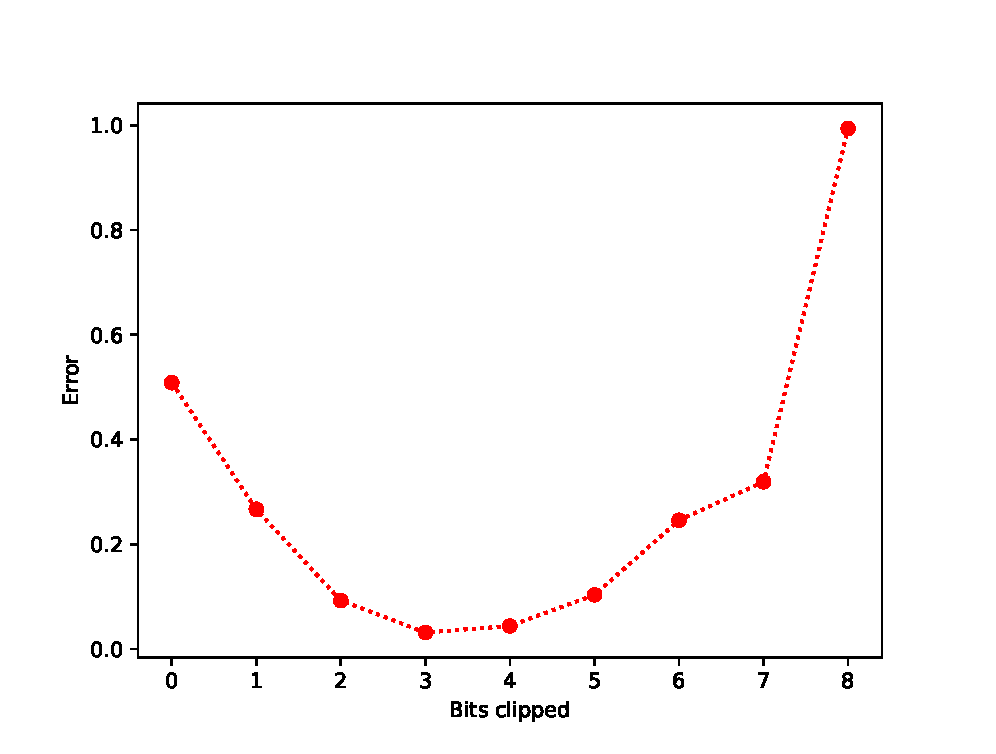
\includegraphics[width=0.85\linewidth]{img/clipping.eps}
  \caption{Simulation of the effect of different result clippings to the layer.}
  \label{fig:clipping}
\end{figure}

A secondary problem cause by the limited bit-width of the DLA relates the bias. Some DNN models rely on bias values close to the maximum value of a signed 32-bit value. This is a problem for the DLA since, it only supports bias values up to 16-bits. This causes some results channels to lose their relative values to equalized due to bias values getting saturated, when the bias values are larger than the maximum 16-bit values.

\section{Board Support Package}
\label{sec:software_support}
We started the actual software development by writing a simple BSP for Headsail. Doing this simultaneously with refining the virtual prototype helped us better understand the complete structure of the SoC.

The BSP is written in \texttt{no\_std} Rust, since it is familiar to the team and has been found effective for rapid collaborative firmware development. Rust has a healthy embedded software ecosystem, with libraries supporting \texttt{no\_std} environments, like our target hardware. Most importantly a community crate called \textsc{riscv-rt}~\cite{riscv_rt}, which is a library that provides startup code and interrupt functionality for bare-metal RISC-V devices.

The Headsail-BSP implements some basic drivers to interact with the hardware's I/O functionality with peripheral UART and CPUs internal timers. BSP also enables interrupts for both CPUs with the CLINT and PLIC peripherals. We also implement basic test bench definitions to enable consistent automated testing setup for CI/CD.

Rust features allow us to host both HPC and SysCtrl specific code in one code base with minimal effort. This allows us to use same peripheral drivers with CPU specific memory maps, reducing the amount of duplicated code. Conditional compilation with Rust feature flags enables us to choose between HPC or SysCtrl builds, to target a specific CPU. Similarly, we can isolate VP and ASIC specific implementations behind their own feature flags.

\subsection{HPC initialization}
Before we can execute binaries on HPC we need to turn it on and initialize it from SysCtrl. For this purpose we run a small \texttt{HPC-init} binary on startup. The initialization program enables the interconnect between the CPUs and turns on the cores of HPC. In addition to turning on HPC it enables and configures most of the peripherals, such as the SDRAM, DLA and clocks.
We provide the initialization program as a part of Headsail-BSP, and have plans to integrate it into an SPI based SD-card boot flow to enable easier workflow with the SoC.
On headsail-vp \texttt{HPC-init} isn't run at all since all the peripherals are configured automatically during startup, making this procedure specific to the ASIC.

\subsection{Dynamic Memory Allocation}
Embedded applications often rely on just statically allocated memory, this makes memory management simple and generally performant. The nature of neural workloads is such that we need the ability to dynamically allocate and free memory. Specifically, we want to be able to dynamically allocate input and output buffers for layers. Since layers have different sized inputs and outputs with large amount of elements, it isn't feasible to statically allocate them all.

Since we support two different programming languages, we had to have solution for both. For C this was accomplished by porting Newlib, which we discuss in detail in section~\ref{sec:newlib}. For Rust we experimented with different possibilities but settled on using an external library called Good Memory Allocator~\cite{galloc_memory_allocator}, which uses bins holding different sized chunks that can dynamically be allocated. Since Good Memory Allocator only depends on the Rust core library, not requiring the full standard library and has been well tested, it suited our purposes well.

\subsection{Memory Map and RISC-V code models}
The CPUs in Headsail--SysCtrl and HPC--work on a semi-unified memory map trough two interconnects. One 32-bit interconnect and one 64-bit interconnect, which allows both of the CPUs to reach external memory regions. The semi-unified comes from the fact that even though the CPUs can both access the same memory regions with same addresses, HPC accesses need to be appended with an extra bit to signify external memory access. This extra bit has the unfortunate effect that it makes every external memory access 64-bits. This mandates that the C-compiler needs to support \texttt{medany} code model~\cite{sifive_riscv_code_models}, which not all instances of riscv-gcc support.

The code model dictates which memory addresses the binary can be mapped to. On RISC-V the standard code model is \texttt{medlow} which enables the code to be linked in a 2 gigabyte long region starting from address $0x0$. Since all external accesses from HPC start with 33rd bit set as one, it would be impossible to link any HPC program to memory outside of it's bootram. Thus, we need to use \texttt{medany} code model which enables using any 2 gigabyte continuous region of memory.

The disadvantage that comes from using \texttt{medany} code model is that it prevents certain linker relaxations from being performed, which in turn negatively affects the performance of the system. In our testing we observed up to a 5 percentage drop in performance when switching from binary linked with \texttt{medlow} to \texttt{medany} when targeting HPC's bootram.

\section{DLA Driver}
To make interfacing with the DLA possible we wrote a driver for the accelerator as a part of the Headsail-BSP, which we simply call the DLA driver.
The driver is implemented as separate Rust module which can be included with the rest of the BSP using optional feature flags, when invoking the build. This is done so that we can reduce the size of the BSP binary when application don't need the DLA. The driver for the DLA is divided into two parts. First is the lower level API that handles the register level interfacing with the DLA. Second is the high-level API which implements a user facing interface for the main operations of the DLA.

\subsection{Layer struct}
The layer configuration struct is the central component of the DLA driver. It defines all the necessary information needed to run a single layer on the DLA and is passed for the \texttt{init\_layer} method in the low level API to run the specified layer. The DLA doesn't wait for a particular run command, rather after setting \texttt{READ\_A\_VALID} and \texttt{READ\_B\_VALID} bits in the \texttt{BUF\_CTRL} register to signal all input and kernel data has been set, the DLA starts immediately executing the current configuration.

\begin{figure}
  \centering
\begin{lstlisting}[language=Rust, basicstyle=\footnotesize, caption={Example call to DLA high-level API}, label={lst:layerstruct}]
pub struct LayerConfig {
  pub input_bank: Option<MemoryBank>,
  pub kernel_bank: Option<MemoryBank>,
  pub output_bank: Option<MemoryBank>,
  pub bias_addr: Option<u32>,
  pub pp_enabled: bool,
  pub relu_enabled: bool,
  pub bias_enabled: bool,
  pub input_size: Option<InputSize>,
  pub kernel_size: Option<KernelSize>,
  pub padding: Option<Padding>,
  pub stride: Option<Stride>,
  pub mac_clip: Option<u32>,
  pub pp_clip: Option<u32>,
  pub simd_mode: Option<SimdBitMode>,
}
\end{lstlisting}
\end{figure}

Program~\ref{lst:layerstruct} shows the design of the struct. The first three fields control the data locations with the DLA memory banks. It should be noted that the driver nor the DLA don't enforce any kind of overlapping protection for the data, and it's left at the responsibility of the user to make sure these areas don't overlap. To make this easier the driver offers a method to calculate suitable memory bank assignments. Bias is handled differently from the other data locations since DLA view it as FIFO where every channel takes the next element.

The \texttt{pp\_enabled}, \texttt{relu\_enabled}, \texttt{bias\_enabled} fields control the use of the post-processing unit. The first enables the unit, and the following ones choose which of the two post-processing operations are executed for the layer. For example when calculating basic Resnet layer with both operations all the three fields need to be enabled.

The \texttt{input\_size}, \texttt{kernel\_size}, \texttt{padding} and \texttt{stride} fields control the dimensions of the 2D convolution. \texttt{input\_size} and \texttt{kernel\_size}, define the height and width of the inputs and weights as well as the channels counts. Number of input channels for input and number of output channels for the kernel. \texttt{padding} fields allows for specifying the amount of padding for all directions separately as well as the values used as the padding. \texttt{stride} tells the amount of space between samples in the input in vertical and horizontal direction separately. The default stride of 1 means that every input element is sampled, whereas stride of 2 means that after a sample, we move two spaces to the particular direction etc. The \texttt{mac\_clip} and \texttt{pp\_clip} fields specify the amount of clipping per operations stage. And finally \texttt{simd\_mode} specifies the use of SIMD operations.

% \begin{figure}
% \centering
% \begin{tikzpicture}[scale=0.7]

% %d Stride 1x1
% \foreach \x in {0, 1, 2, 3} {
%   \foreach \y in {0, 1, 2, 3} {
%       \draw[black, thick] (\x,\y) rectangle (\x+1,\y+1);
%       \fill[blue!20] (\x,\y) rectangle (\x+1,\y+1);
%   }
% }
% \node[below] at (1.5, -0.5) {Stride 1x1};

% % Stride 1x2
% \begin{scope}[shift={(6, 0)}]
%   \foreach \x in {0, 1, 2, 3} {
%       \foreach \y in {0, 1, 2, 3} {
%           \draw[black, thick] (\x,\y) rectangle (\x+1,\y+1);
%       }
%   }
%   \foreach \x in {0, 1, 2, 3} {
%       \foreach \y in {0, 2} {
%           \fill[blue!20] (\x,\y) rectangle (\x+1,\y+1);
%       }
%   }
%   \node[below] at (1.5, -0.5) {Stride 1x2};
% \end{scope}

% % Stride 2x2
% \begin{scope}[shift={(12, 0)}]
%   \foreach \x in {0, 1, 2, 3} {
%       \foreach \y in {0, 1, 2, 3} {
%           \draw[black, thick] (\x,\y) rectangle (\x+1,\y+1);
%       }
%   }
%   \foreach \x in {0, 2} {
%       \foreach \y in {0, 2} {
%           \fill[blue!20] (\x,\y) rectangle (\x+1,\y+1);
%       }
%   }
%   \node[below] at (1.5, -0.5) {Stride 2x2};
% \end{scope}
% \end{tikzpicture}
% \caption{Effect of stride to sampling}
% \label{fig:stride}
% \end{figure}

\subsection{Reading Layer Results}
To get output from the DLA we first need to define the output address. This address can be any memory address visible to the control processors, but in the driver we have a limited the number of possible output addresses only to the DLA's internal memory banks. For setting the output bank for the given layer the driver writes to \texttt{DLA\_PP\_AXI\_WRITE\_ADDRESS} register the wanted output address.

To read the output from the DLA we need to know how many elements the output has for any given operation. This information can be derived from the following equation

\begin{equation}
W_{\text{out}} = \frac{W_{\text{in}} + P_{\text{left}} + P_{\text{right}} - K_x + 1}{S_x}
\end{equation}
\begin{equation}
H_{\text{out}} = \frac{H_{\text{in}} + P_{\text{top}} + P_{\text{bottom}} - K_y + 1}{S_y}
\end{equation}
\begin{equation}
\text{No. output elements} = W_{\text{out}} \cdot H_{\text{out}} \cdot Channels_{out},
\end{equation}
where $W$ is width, $H$ is height, $P$ is padding to either left, right, bottom or top, $K$ is the shape of the kernel and $S$ is the stride in horizontal or vertical direction.
Multiplying the shape of a single output channel with the total number of output channels gives use the total amount of output elements. Since DLA can only output 8-bit values we know that the number of bites to read per layer is equal to the amount of output elements.

As explained in section~\ref{sec:result-width-problem} the output of the DLA is limited to the signed 8 bit range (from $-128$ to $127$) but the convolution is calculated in signed 16-bit range (from $-32768$ to $32767$) the DLA needs to clip half of the bits away. Using the \texttt{mac\_clip} and \texttt{pp\_clip} fields we can control which of the consecutive 8-bits we want to use as the result. By default, DLA stores the 8 least significant bits, but by increasing the clipping values we can move the extraction window towards the more significant bits. By moving towards LSB we essentially gain granularity between the values at the cost of losing range in the high values. This is desired when the absolute maximum value of a layer is small. In most cases the optimal extraction window is somewhere between MSB and LSB, thus making it difficult to predict which exact clipping value to use. When the results of a layer are read from the DLA the driver shifts the read values back by the same amount as they were clipped in the accelerator to match the magnitude of the calculations.

To find an optimal clipping amount for each layer, we propose a bias maximum value based heuristic
\begin{align}
P & = \max \left( \log_{2} \left( \frac{\max \left( \mathopen| \max(\hat{b}) \mathclose|, \; \mathopen| \min(\hat{b}) \mathclose| \right)}{127} \right), \; 127 \right) + 1 \\
  & \text{Bits clipped} =
  \begin{cases}
    P, &  \text{for} \; P < 8  \\
    8, &  \; \text{otherwise}
  \end{cases}
\end{align}
where $\hat{b}$ is the vector containing all the bias values associated with a given layer. From this vector we find the value with the greatest absolute value, and choose the number of bits needed to represent it as the amount of clipping to use incremented by one. In out testing this heuristic somewhat improved the predictions results when compared to choosing a static amount of clipping.
We limit the number of clipped bits to high of 8 since, the bit width of the convolution result is 16-bits.


\subsection{C-Interface}
To enable TVM BYOC to call the DLA drivers high-level interface we needed to create C-wrappers for the function calls. This was done by implementing a Foreign Function Interface (FFI) for the Rust function calls with the Cbindgen library~\cite{cbindgen}. Cbindgen generates C headers from the Rust code that enables C programs to call Rust functions when linked with the proper static library. For the static library we build the headsail-bsp that implements the high-level operation calls which the FFI interface uses.

In the FFI we also define a entry point specifically for the TVM. As previously mentioned we always allocate \texttt{qnn.conv2d} + \texttt{add} pattern for the DLA to execute. The code generation backend extract all the necessary information from the Relay nodes of this pattern and generates a function call to call \texttt{dla\_tvm\_qnn\_conv2d\_bias} function from the FFI. In addition to just calling the wanted Conv2D + bias operation from the BSP, the FFI function slices the data buffers to Rust slices and performs certain value conversions, like clipping the 32-bit bias values to 16-bit values. After the operation has been done and the result rest the FFI implementations shifts the values left by the same amount as was clipped in the DLA. These values are then copied to the buffer defined by the TVM codegen.

\section{Porting Newlib}
\label{sec:newlib}

\begin{table}[]
\centering
\begin{tabular}{|l|l|c|}
\hline
\textbf{Syscall}       & \textbf{Description}               & \textbf{Implemented} \\ \hline
\texttt{exit}         & Terminates the process             & \scalecheck                       \\ \hline
\texttt{close}         & Closes a file                      &                        \\ \hline
\texttt{fstat}         & Gets file status                   & \scalecheck                       \\ \hline
\texttt{getpid}        & Gets the process ID                &                        \\ \hline
\texttt{isatty}        & Tests if a file descriptor is a terminal & \scalecheck                 \\ \hline
\texttt{kill}          & Removes a process                    &                        \\ \hline
\texttt{link}          & Creates a hard link to a file      &                        \\ \hline
\texttt{lseek}         & Re-positions read/write file offset &                        \\ \hline
\texttt{open}          & Opens a file                       &                        \\ \hline
\texttt{read}          & Reads from a file                  & \scalecheck                       \\ \hline
\texttt{sbrk}          & Moves end of heap pointer          & \scalecheck                       \\ \hline
\texttt{stat}          & Retrieves file status              &                        \\ \hline
\texttt{times}         & Returns process times              &                        \\ \hline
\texttt{unlink}        & Deletes a name or a file           &                        \\ \hline
\texttt{wait}          & Waits for process to change state  &                        \\ \hline
\texttt{write}         & Writes to a file                   & \scalecheck                       \\ \hline
\end{tabular}
\caption{Newlib Syscalls and Implementation Status}
\label{tab:newlib_syscalls}
\end{table}
Since we wanted to use TVM's AOT runtime to execute inference in the benchmark we had to provide it with a C standard library implementation. For this purpose we chose to port Newlib for Headsail, since it's known to be relatively easy to adapt for new platforms.

Newlib is an implementation of the C standard library meant for use in embedded devices~\parencite{newlib}. It is separated into two different parts. First is the Newlib core which implements the actual standard library for different CPU ISA's. Since Newlib already has support for RISC-V we didn't need to modify Newlib core in any way. Second part of Newlib is called Libgloss, which implements the platform dependent features. For this port we decided to only implement the minimum required functionalities of Libgloss.

\begin{figure}
\begin{lstlisting}[language=C, caption={Minimal implementation of the fork() syscall in Newlib Libgloss}, label={lst:newlib-stump}]
int _fork() {
    return -1;
}
\end{lstlisting}
\end{figure}

Porting Libgloss involves implementing 16 system calls, crt0 and a linker script. From the 16 system calls only some are mandatory for us to implement, because we are targeting only bare-metal applications without a filesystem. The table~\ref{tab:newlib_syscalls} shows all the Libgloss system calls with column 3 displaying if we implemented the call. The unimplemented calls still need to be defined in the Libgloss source for linking purposes, but they don't need to do anything except return an error. Program~\ref{lst:newlib-stump}, shows and example of a minimal implementation for the fork system call in Headsail's Newlib port. The purpose of the Fork system calls is to  duplicate a process, but since we don't support multithreading or any other form of process concurrency it will never be called, thus having it return error is correct behaviour. We use this same approach in the rest of the system call that we didn't implement.

The system calls can be implemented either in non-reentrant or reentrant way. Re-entrant system calls are thread safe but require an additional argument--the reentrancy structure--to be passed. Reentrancy structure holds local values specific for that instance of the function call, whereas the non-reentrant version of the function refers to shared global variables. For single threaded applications on Headsail implementing the non-reentrant systems calls was enough.~\parencite{bennett2010porting}

In addition to the system calls Libgloss needs to have a crt0, which is a small program that includes a \texttt{\_start} symbol, a call to the \texttt{main} function, some global definitions, and optionally hardware initializations. The \texttt{\_start} symbol signifies the beginning of a C program and is used by the linker to place the program to start from the correct memory address. After declaring the \texttt{\_start} symbol, our crt0 clears the bss segment, registers the \texttt{exit} function, initializes the UART and finally calls the \texttt{main} function.

\begin{figure}[h]
\centering
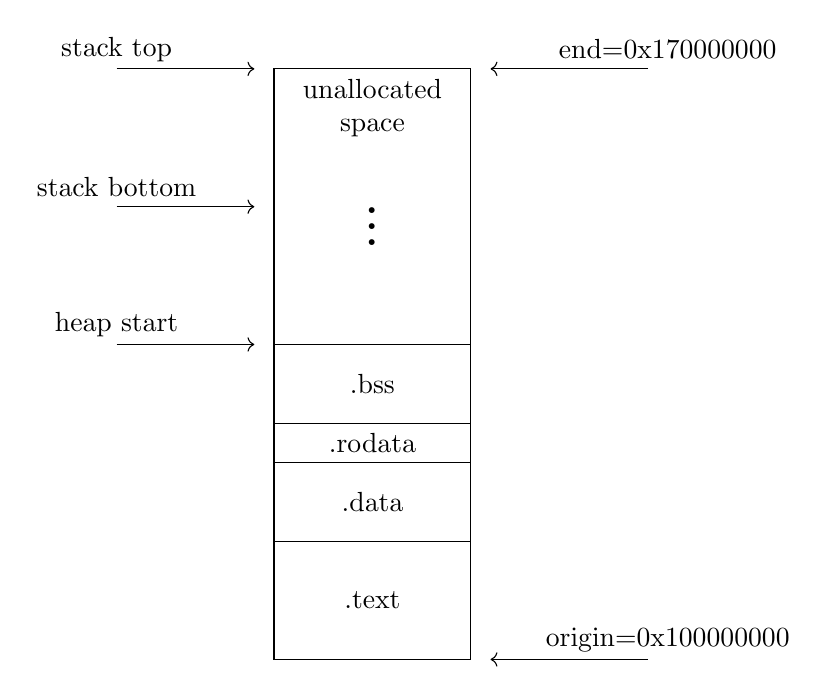
\begin{tikzpicture}[scale=0.5]
\draw (0, 0) rectangle (5, 3) node[midway] {.text};
\draw (0, 3) rectangle (5, 5) node[midway] {.data};
\draw (0, 5) rectangle (5, 6) node[midway] {.rodata};
\draw (0, 6) rectangle (5, 8) node[midway] {.bss};
\draw (0, 8) rectangle (5, 15);
\node at (2.5, 14.5) {unallocated};
\node at (2.5, 13.5) {space};
\node[scale=2] at (2.5, 11) {.};
\node[scale=2] at (2.5, 11.4) {.};
\node[scale=2] at (2.5, 10.6) {.};
\node at (10, 0.5) {origin=0x100000000};
\node at (10, 15.5) {end=0x170000000};
\node at (-4, 15.5) {stack top};
\node at (-4, 12) {stack bottom};
\node at (-4, 8.5) {heap start};

\draw[->] (9.5, 0) -- (5.5,0);
\draw[->] (9.5, 15) -- (5.5,15);
\draw[->] (-4, 11.5) -- (-0.5, 11.5);
\draw[->] (-4, 15) -- (-0.5, 15);
\draw[->] (-4, 8) -- (-0.5, 8);
\end{tikzpicture}
\caption{Example configuration of linked program in memory}
\label{fig:sdram-memory-layout}
\end{figure}

The linker script is the final component needed by the Libgloss. It tells the linker how to link the object files produced by the compiler. Our linker script maps the whole SDRAM on Headsail as it's total available memory region, which it then splits into the text section, data and read-only data sections and various different initialization sections. Additionally, the linker reserves space for the stack and heap data structures according to the linker script definitions. Figure~\ref{fig:sdram-memory-layout} shows an example of how a binary is placed in to the Headsail's SDRAM according to the defined linker script. We always place the \texttt{\_start} start symbol at the beginning of the SDRAM, followed by data sections. By default, the linker allocates 4 megabytes to the stack and rest is allocated to the heap. The allocations are controlled by specific flags defined in the linker script, that are visible to program.


\section{TVM transformation scheme and code generation}
After trial and error we settled on a TVM graph transformation behaviour that provided us with the most stable results in all the tested models. With the implemented graph transformations we were able to assign any Conv2D + bias pattern using INT8 parameters to be executed on the DLA.

We implemented our own QNN legalization pass for TVM, in which we look for a TVM canonicalized version of a TFlite quantized conv2d fusion layer. In TVM Relay representation this pattern is composed of 4 nodes: \texttt{qnn.conv2d}, \texttt{nn.bias\_add}, \texttt{qnn.requantize}, and \texttt{clip}. We also capture an optional pair of nodes at the end of main block. If the fusion layer is followed by \texttt{qnn.add} and \texttt{clip} we capture those nodes as well. This combination is seen in ResNet architecture as the operations to concatenate main branch and the skip branch.

From the found pattern we remove all the zero point corrections from \texttt{qnn.conv2d} and \texttt{qnn.requantize} nodes, if they are present. We learned that the TFlite models offered by MLPerf Tiny tended to use affine quantization with zero point being close to $128$. Value this high doesn't work for Headsail DLA, since all base values over $0$ would get clipped.
We also remove the zero point from the optional skip connection concatenation node if it was captured, even if the operation is not assigned to the accelerator.

After legalization we do pattern matching for two patterns. First is the standard 2D convolution followed by bias and second is grouped convolution followed by a bias. These patterns are assigned to be executed on the DLA using the high-level API symbols from the FFI. Since TVM doesn't separate between grouped and non-grouped convolutions we use the \texttt{groups} parameter in the \texttt{qnn.conv2d} as a metric to distinguish the two. If the number of groups is more than $1$, we annotate the pattern as grouped convolution.

In the code generation backend we traverse the legalized graph and operate on all the patterns that have been assigned for execution on the DLA.
From each pattern we extract the embedded operation parameters to produce valid C code to call the high-level API operations. We also generate code to dynamically allocate memory for the intermediary results.
Some of the operation parameters need to be dynamically extracted from the graph information.

Appendix A shows an example of the code generated for one convolution layer with the Headail TVM backend. First we include all the necessary libraries to each generated file. Then we generate the function definition that takes four parameters, from the AOT runtime. The first two are the buffers for layer input and weights, third one is the bias FIFO buffer, and last one is the result buffer for that layer.
The body of the function consists of allocating an intermediary buffer for the results. This is needed in where we have multiple sequential convolutions in a row, which is not the case in this example.
Next we have the actual API call which gets as its parameters all the necessary information extracted from the original graph representation of the layer. Finally, we copy the result of the operation from the intermediary buffer to the runtime output buffer and free the intermediary buffer. TVM AOT runtime expected each external codegen call to return a 0 upon successful completion.

\section{Benchmarking}
For the DLA there are two things we can benchmark. First is to look at the amount of convolution operations we can execute per time unit. This kind of throughput benchmarking is fine but doesn't tell us much about the real-life CNN performance, since it doesn't take into an account what proportion of the CNN workloads is actually Conv2d and the proceeding Bias and ReLU operations.

The second option is to model real-life use-cases of CNNs and benchmark the inference latency of the models. For this purpose we chose to use MLPerf Tiny Benchmark~\cite{tinyperf} from MLCommons, which we describe in detail in section~\ref{sec:tinyperf}.
From these benchmarks the anomaly Detection is unacceleratable with the Headsail DLA since it uses FC-AutoEncoder network, which is based on fully connected layers and thus has no operations which our accelerator can execute.

\begin{figure}[h]
\centering
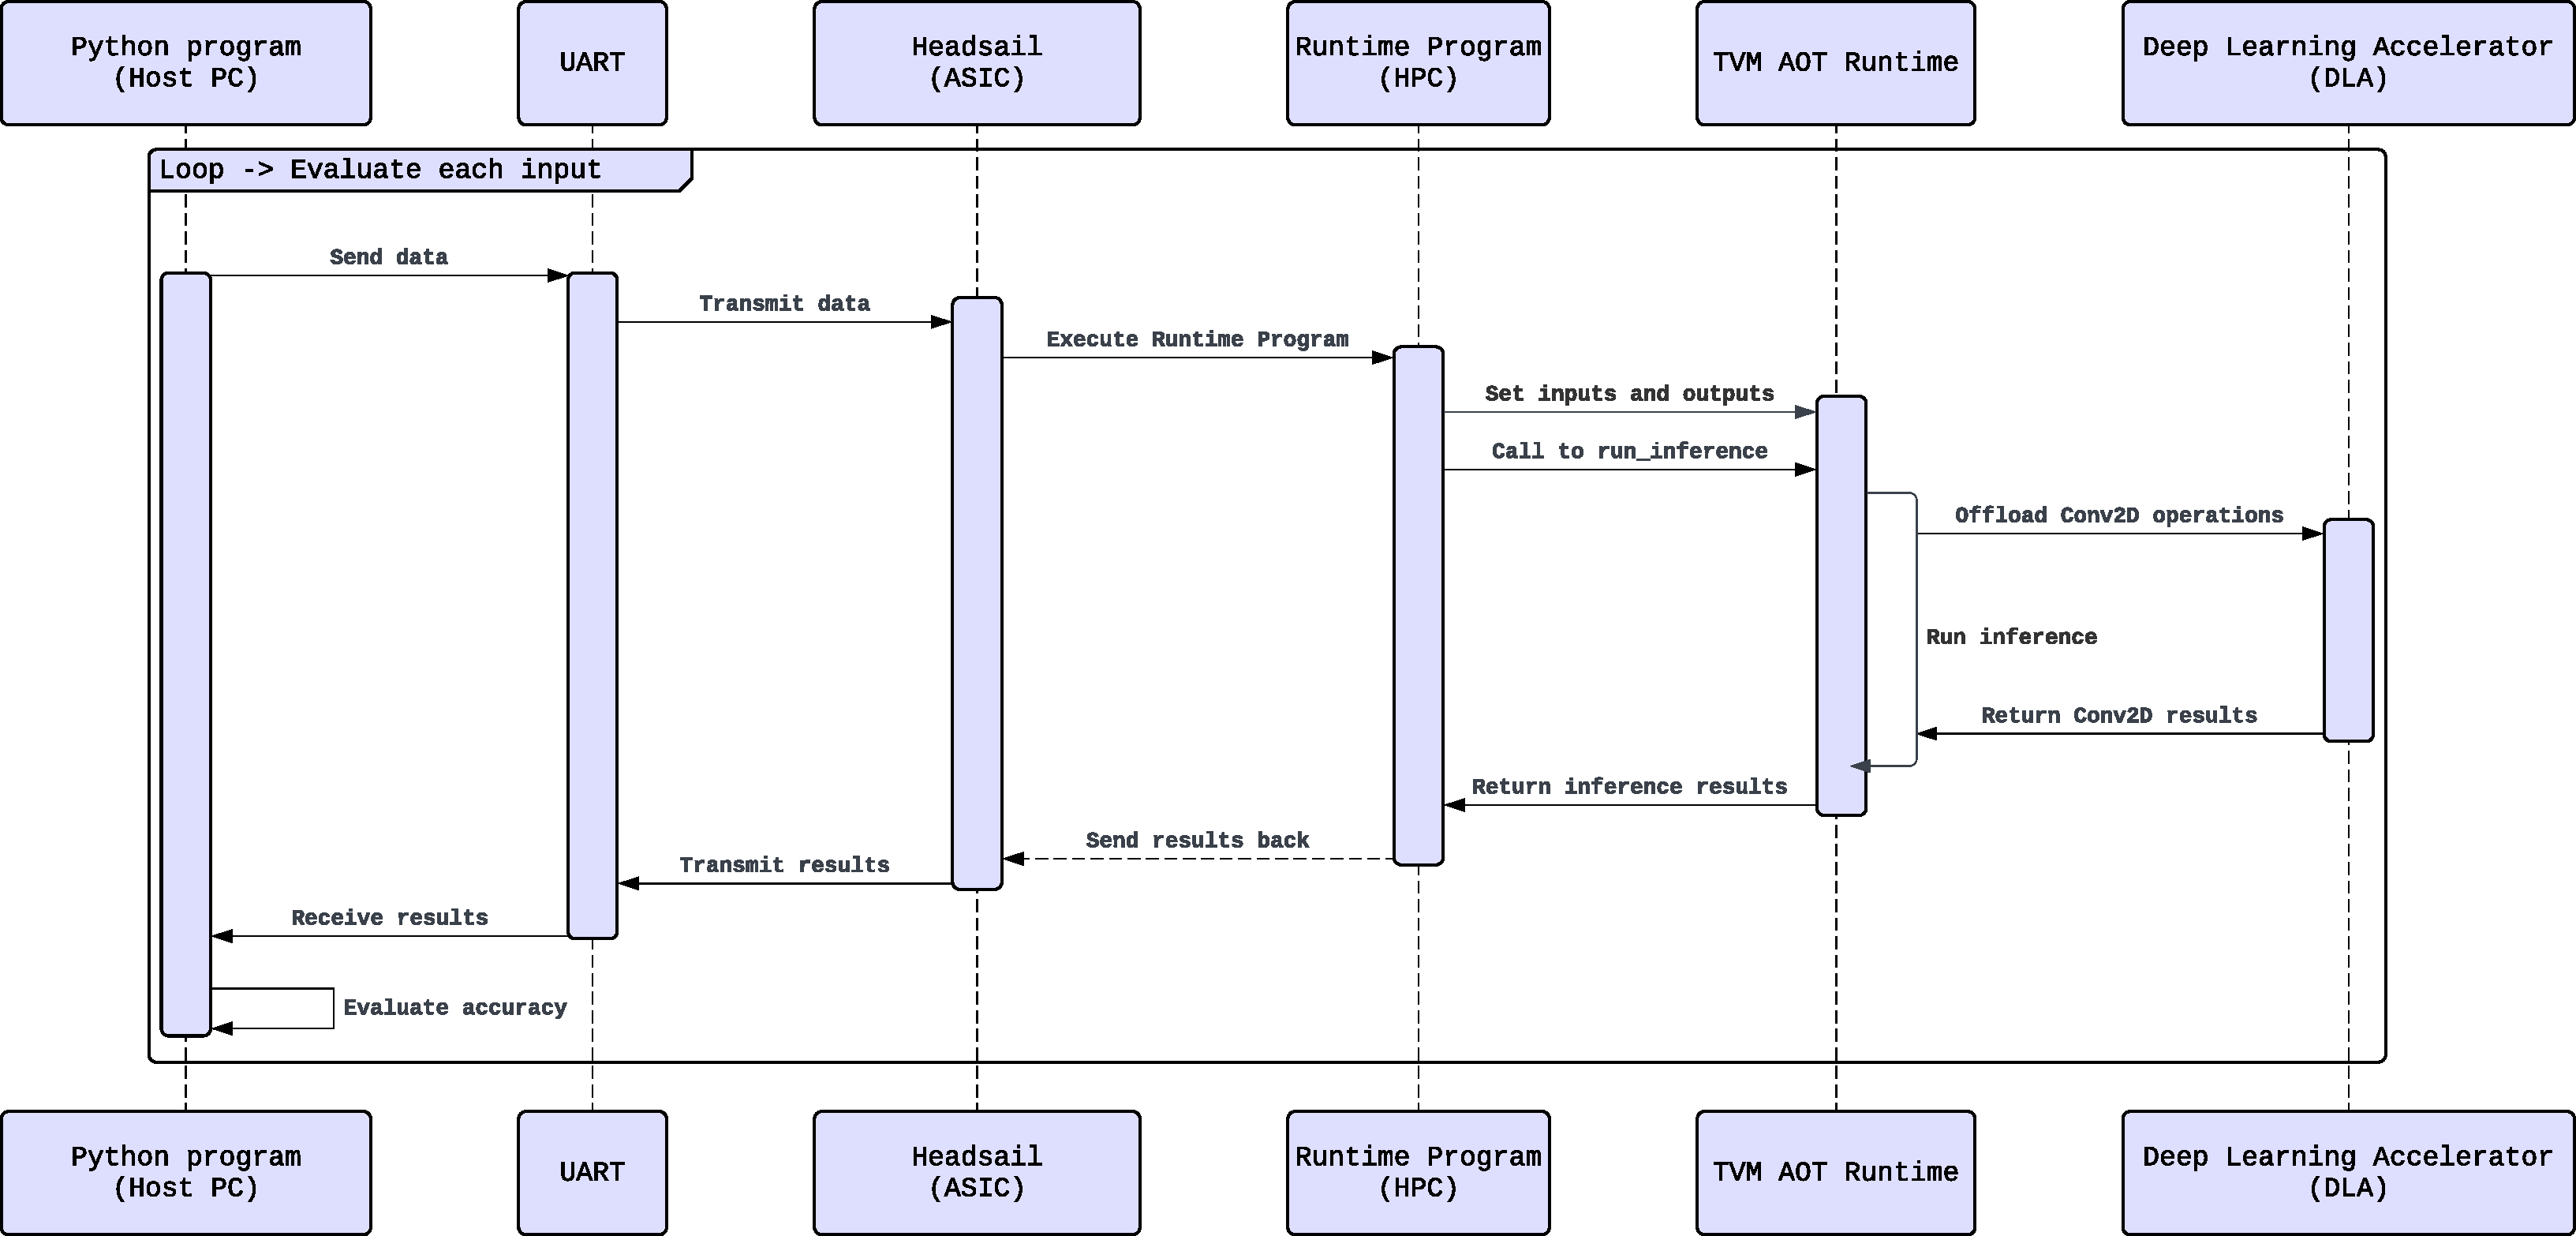
\includegraphics[width=\linewidth]{img/benchmark-sequence.pdf}
\caption{Sequence diagram for MLPerf Tiny benchmarking on Headsail.}
\label{fig:dla_sequence}
\end{figure}

Figure~\ref{fig:dla_sequence} shows the sequence of running the MLPerf Tiny benchmark on Headsail. We use a simple Python program running on a host PC as the runner, which reads the benchmark samples from the dataset and send them to Headsail over UART. Since MLPerf Tiny only measures the performance of actual inference, we decided to use the relatively slow UART over SPI or I2C for the simplicity. HPC on Headsail runs a simple C-program to receive the data over UART and to set that data as input for the TVM AOT runtime. After setting the input and output the program calls the AOT runtime API to run inference for the given sample. AOT runtime then sequentially executes the model graph with the annotated graph patterns allocated for the DLA. Result of the inference is then transmitted over UART to the host PC, where the Python program receives it, finds the top-1 classification from the vector and updates the evaluation metric, before sending the next input for inference.

We also want to compare how the DLA compares to running the same benchmark without the accelerator. To do this we can invoke the TVM AOT runtime to be built without graph annotations, allocating all the convolution to HPC. This is necessary to conclude if the accelerator is actually able to accelerate the workloads meant for it.

The results of this benchmarking serve two purposes. First is to evaluate the suitability of the DLA for executing pretrained INT8 quantized models. In an ideal case DLA can take any arbitrary quantized CNN and improve its inference performance in comparison to just running it on the HPC. If the DLA reaches accuracies close to the ones of the reference models, we would consider it a success.
The second purpose of this benchmark is to actually evaluate the performance of the HPC and the DLA ASIC in CNN workloads.

\section{Complete DLA Software Architecture}
\begin{figure}
\centering
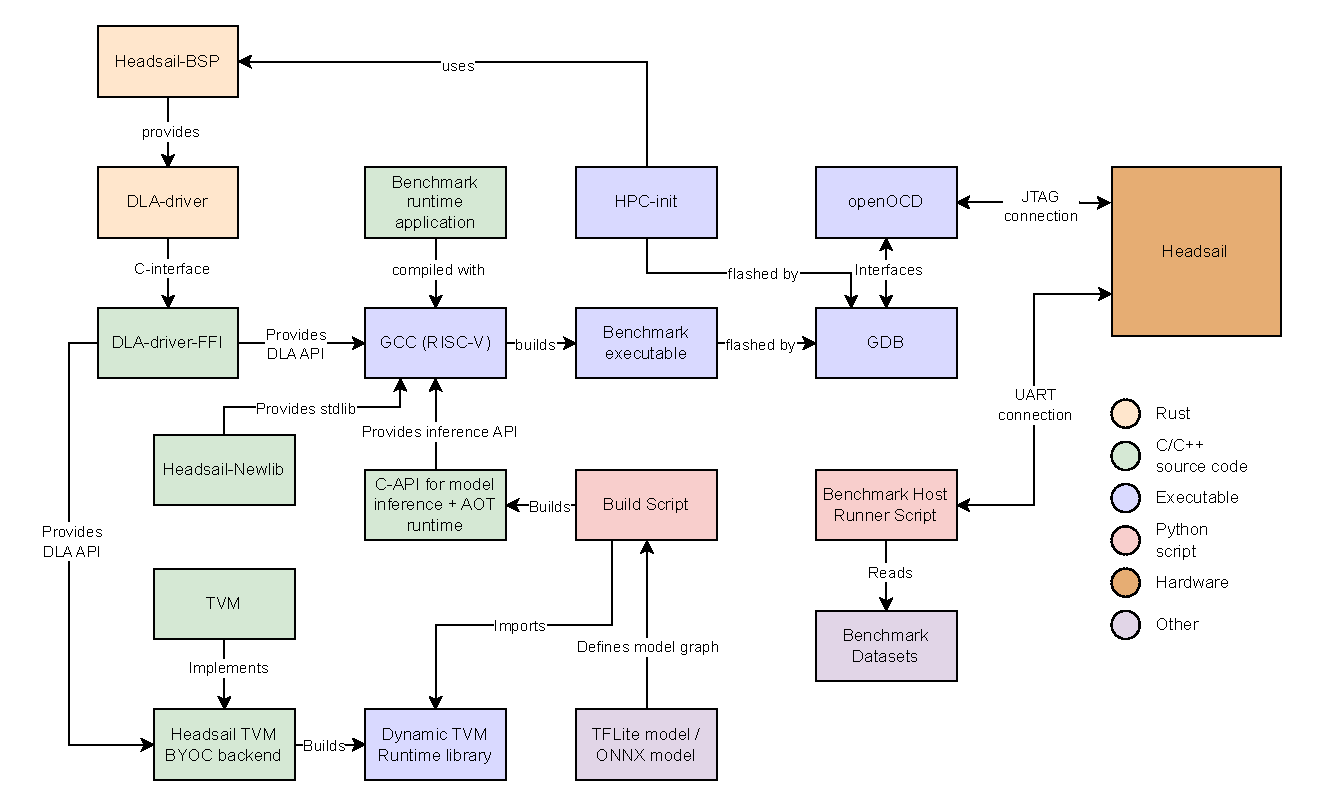
\includegraphics[width=\linewidth]{img/dla-architecture-new.pdf}
\caption{Software architecture of accelerated DLA flow in Headsail with TVM runtime and a TFlite model}
\label{fig:architecture}
\end{figure}

The figure~\ref{fig:architecture} presents the software architecture of TVM annotated model deployment flow with Headsail DLA. The end goal of this flow is to build and executable binary that includes the AOT runtime with one of the MLPerf Tiny models to run inference on samples received over UART. The build flow is orchestrated with CMake and the model code generation with a Python script.

The first part of the build process is the TVM code generation. We read the targeted TFlite model with a Python build script and import it to TVM Relay graph.
TVM then performs QNN-legalization pass for the graph defined in the Headsail's Python API and assign the defined patterns for execution on the DLA, producing a DLA compatible relay graph.
This graph is then compiled to C source code with the TVM dynamic runtime which has been compiled with support for Headsail BYOC backend, which uses the symbols from DLA-driver's C-interface to execute the CNN operations. The DLA directives are embedded into the AOT graph to produce complete pipeline for executing inference on the specific model. This source code is then linked with our standard library implementation, the runner application and DLA-driver using riscv64-unknown-none-elf compiler stack to produce an executable binary that can be run on HPC.

Both of the CPUs in the Headsail are equipped with JTAG connectors which we can connect to with OpenOCD~\cite{openocd2023}. We configure OpenOCD to provide us with a GDB~\cite{gdb2023} interface, which we use to flash the executables. First we run HPC's initialization code on SysCtrl to turn on HPC and all the necessary peripherals, after which we can flash the benchmark executable onto HPC and begin the benchmark.

Running the benchmark is done with simple Python script which reads one input from the targeted benchmark task at a time and writes them to Headsail over UART for inference.
The script then waits for the runner program on Headsail to respond with the result vector of the inference, from which it finds the top-1 classification and updates the precision score for the benchmark, before sending the next input.

Even though Headsail is the third SoC Hub SoC, it had little existing software support for C that could utilize the SoC specific features like UART. So a major part of this project involved setting up a Headsail compatible C-toolchain. Since Headsail has RISC-V CPUs we could use an already existing riscv-gnu-toolchain for the compiler, but we still had to set up a C standard library for the chip with custom version of Newlib Libgloss. Also, due to specific memory addressing decisions in the hardware, we needed to use \texttt{medany} code model compatible compiler and standard library when targeting the 64-bit processor.



\chapter{Results}
\label{ch:results}
After finishing development of the software stack described in the chapter~\ref{ch:implementation} we ran the MLPerf Tiny benchmark for two configurations. First being on the headsail-vp with only single HPC core, and second on headsail-vp with single HPC core and the DLA-vp working in tandem. Unfortunately due to problems with the ASIC, we were not able to include any results from the hardware and thus this benchmark only serves the purpose of validating the ability of headsail-vp to execute the reference models.
\begin{table}[h]
\centering
\begin{tabular}{|l|l|c|c|c|c|}
\hline
  \multirow{2}{*}{\textbf{Task}}  & \multirow{2}{*}{\textbf{Target}}  & \multirow{2}{*}{\shortstack[c]{\textbf{Accuracy}\\ eq.~\ref{eq:accuracy}}} & \multirow{2}{*}{\shortstack[c]{\textbf{Precision}\\ eq.~\ref{eq:precision}}} & \multirow{2}{*}{\shortstack[c]{\textbf{Recall} \\eq.~\ref{eq:recall}}} & \multirow{2}{*}{\shortstack[c]{\textbf{Passes}\\ \textbf{MLPerf Tiny}}} \\
  & & & & & \\\hline
\multirow{2}{*}{\shortstack[l]{\textbf{Keyword}\\ \textbf{Spotting (KWS)}}}
                                  & \textbf{HPC} & 0.90               & 0.92       & 0.90     & \scalecheck                          \\ \cline{2-6}
                                  & \textbf{HPC+DLA} & 0.90               & 0.92   & 0.90         & \scalecheck                          \\ \hline
\multirow{2}{*}{\shortstack[l]{\textbf{Image}\\ \textbf{Classifcation (IC)}}}
                                  & \textbf{HPC} & 0.88               & 0.88      & 0.88      & \scalecheck                          \\ \cline{2-6}
                                  & \textbf{HPC+DLA} & 0.69               & 0.74      & 0.70      &                            \\ \hline
\multirow{2}{*}{\shortstack[l]{\textbf{Visual Wake}\\ \textbf{Words (VWW)}}}
                                  & \textbf{HPC} & 0.83               & 0.83        & 0.84    & \scalecheck                          \\ \cline{2-6}
                                  & \textbf{HPC+DLA} & 0.50               & 0.50   & 0.50          &                            \\ \hline
\multirow{2}{*}{\shortstack[l]{\textbf{Anomaly}\\ \textbf{Detection (AD)}}}
                                  & \textbf{HPC } & \multicolumn{3}{c|}{\textbf{AUC} = 0.68}     &   \\ \cline{2-6}
                                  & \textbf{HPC+DLA} & \multicolumn{3}{c|}{-}      &                            \\ \hline

\end{tabular}
\caption{MLPerf Tiny benchmark results for HPC and HPC with DLA.}
\label{tab:benchmark-results}
\end{table}

The table~\ref{tab:benchmark-results} presents the results of the MLPerf Tiny benchmark, for HPC standalone and HPC with two-dimensional convolutions assigned to the DLA. As noted previously the anomaly detection task is unacceleratable due to the lack of two-dimensional convolution layers suitable for execution on the DLA, and thus we have results for HPC only run.

When run without the DLA, just with HPC, Headsail passes the accuracy requirements for all the tasks, except anomaly detection, as can be seen from the last column of the table.
For the runs with DLA performing the convolution operations, only keyword spotting task passed the required accuracy threshold.

As mentioned previously Renode isn't fitting for performance evaluation, and thus it isn't feasible to benchmark DLA-vp with MLPerf Tiny. We can however run the MLPerf Tiny tasks to see if the DLA reaches the required accuracy requirements of the benchmark. This essentially verifies the complete software stack and was especially useful during the development of DLA graph legalization pass.

\section{Image classification}
\begin{figure}[h]
  \centering
  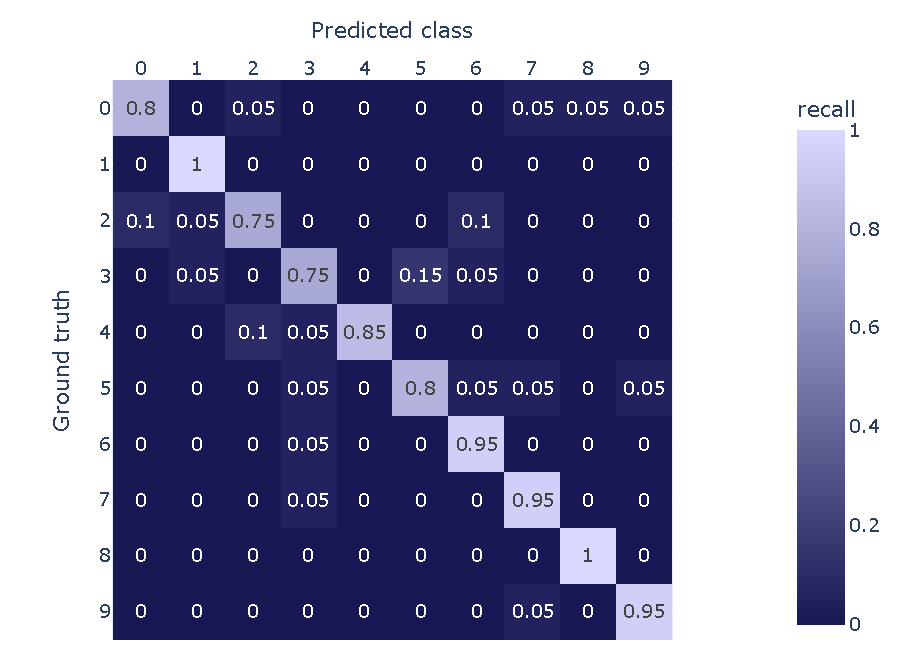
\includegraphics[width=0.8\textwidth]{img/ic_200_no_acc.eps}
  \caption{Confusion matrix of image classification task results without DLA (N=200).}
  \label{fig:ic-results-no-acc}
\end{figure}


\begin{figure}[h]
  \centering
  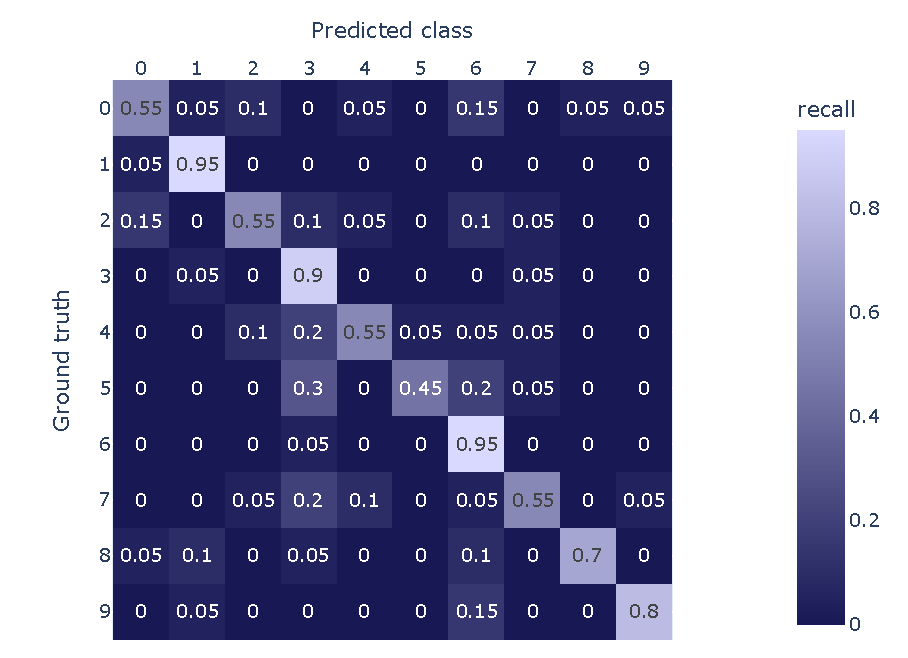
\includegraphics[width=0.8\textwidth]{img/ic_200_abs_heuristic.eps}
  \caption{Confusion matrix of image classification task results when using bias heuristic (N=200).}
  \label{fig:ic-results}
\end{figure}


Figure~\ref{fig:ic-results-no-acc} shows the results for running the IC task without the DLA as a class confusion matrix. With accuracy of $0.88$ it easily passes the
required accuracy threshold of $85\%$ for submitting the IC benchmark scores. This result is inline with reference model, and as mentioned in section~\ref{sec:tinyperf-ic} the evaluation metric for the IC task is Top-1, and thus we are only interested if the inference identified the correct class, no matter what was its confidence on that answer.

Figure~\ref{fig:ic-results} shows the results for the MLPerf Tiny image classification benchmark. From the result we can see that there is a major difference in classification accuracy between classes. Classes $1$, $3$ and $6$ have higher recall than the minimum asked by MLPerf Tiny, but entries in classes $0$, $2$, $4$, $5$ and $7$ are misidentified almost half of the time. With total accuracy of $0.69$ Headsail-DLA doesn't reach the accuracy threshold of the task.

When compared to the runs without the DLA, we can see that there are some similarities in which classes get confused with which classes, but the error seems to get exaggerated with the DLA.
This discrepancy is almost completely explained by the clipping behaviour, since when DLA-vp is modified to output the complete result, this difference between the runs disappears and DLA performs similarly as the HPC only run. Giving us confidence that our approach in the graph transformations is correct and rest of the stack is working correctly.

\section{Keyword spotting}

\begin{figure}[h]
  \centering
  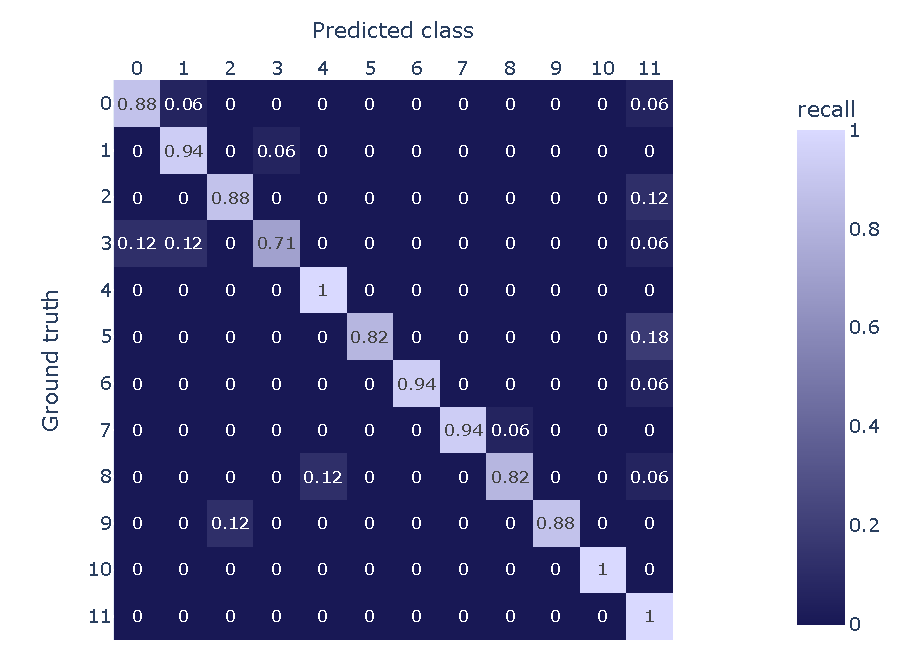
\includegraphics[width=0.8\textwidth]{img/kws_200_no_acc.eps}
  \caption{Confusion matrix of keyword spotting task results without DLA (N=200).}
  \label{fig:kws-results-no-acc}
\end{figure}
\begin{figure}[h]
  \centering
  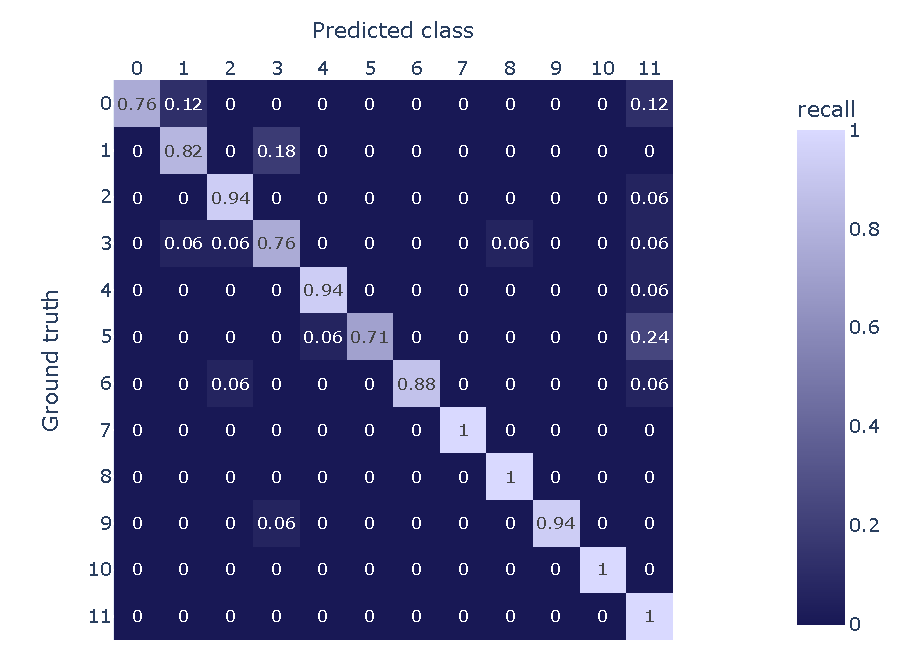
\includegraphics[width=0.8\textwidth]{img/kws_200_abs_heuristic.eps}
  \caption{Confusion matrix of keyword spotting task results when using bias heuristic (N=200).}
  \label{fig:kws-results}
\end{figure}


\noindent Figure~\ref{fig:kws-results-no-acc} shows the results for the MLPerf Tiny keyword spotting benchmark ran on HPC only. Similarly, as with the image classification task the evaluation metric was Top-1 accuracy. The CPU only run of the benchmark performed as expected, reaching the required accuracy of $90\%$, as we expected from the reference model.

Figure~\ref{fig:kws-results} shows the results for the DLA accelerated run. For the keyword spotting the DLA performed well, exactly hitting the $90\%$ minimum accuracy requirement.
Unlike the rest of the benchmark, in this task the DLA performed as well as the unaccelerated run did.

By comparing the two results, we can see that the CPU only run performed more evenly in regard to which classes it could correctly classify, than the DLA run which had more classes it struggled with as well as more classes which it could perfectly classify.

\section{Visual Wake Words}
% \begin{figure}
% \centering
% \begin{minipage}{.45\textwidth}
%   \centering
%   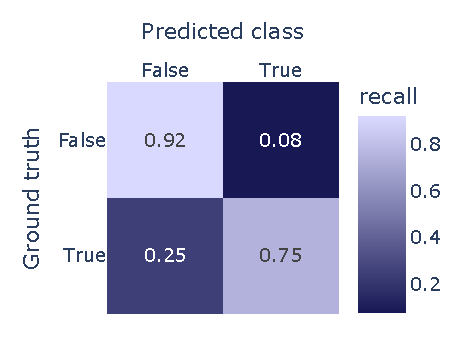
\includegraphics[width=\linewidth]{img/vww_200_no_acc.eps}
%   \caption{VWW task on headsail-vp without DLA}
%   \label{fig:vww-no-acc}
% \end{minipage}
% \begin{minipage}{.45\textwidth}
%   \centering
%   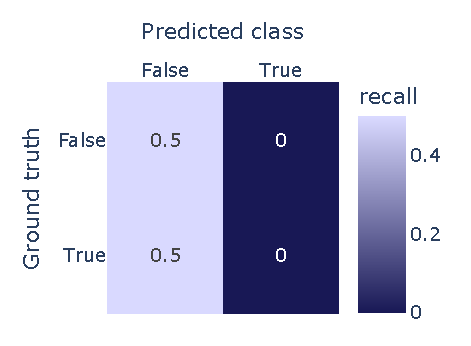
\includegraphics[width=\linewidth]{img/vww_200_acc.eps}
%   \caption{VWW task on headsail-vp with DLA}
%   \label{fig:vww-dla}
% \end{minipage}%
% \caption{Visual wake word task results on Headsail}
% \label{fig:vww-results}
% \end{figure}

\begin{figure}
  \centering
  \begin{subfigure}[t]{0.5\textwidth}
    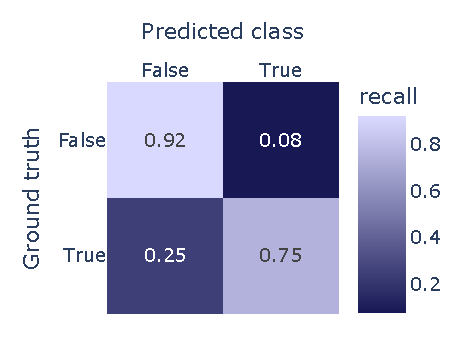
\includegraphics[width=\linewidth]{img/vww_200_no_acc.eps}
    \caption{VWW task on headsail-vp without DLA}
    \label{fig:vww-no-acc}
  \end{subfigure}%
  ~
  \begin{subfigure}[t]{0.5\textwidth}
    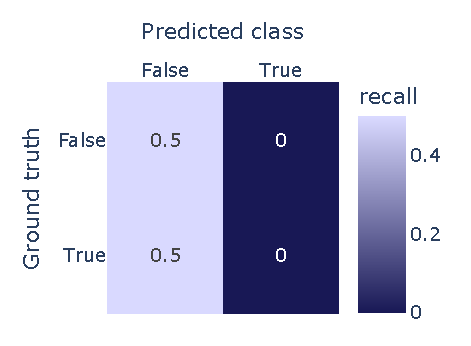
\includegraphics[width=\linewidth]{img/vww_200_acc.eps}
    \caption{VWW task on headsail-vp with DLA}
    \label{fig:vww-dla}
  \end{subfigure}%
  \caption{Visual wake word task results on Headsail}
  \label{fig:vww-results}
\end{figure}


Figure~\ref{fig:vww-results} shows the results of the MLPerf Tiny visual wake word task for headsail-vp. Subfigure~\ref{fig:vww-no-acc} shows the results of the benchmark for the CPU only run. This run exceeds the required $80\%$ accuracy threshold with an accuracy of $83\%$. From the confusion matrix we can see that the reference model has a bias towards false predictions. This effect can be seen exaggerated in the benchmark run with the DLA in figure~\ref{fig:vww-dla}. From the results of the DLA run we can conclude that the MLPerf Tiny reference model is not compatible with the DLA at this point, since accuracy of $0.5$ for a binary classifier implies a random results.

At this moment it's unclear why this task performed so poorly with the DLA, but what we are seeing from the results is that with DLA it's impossible to make a true prediction with this setup. This is supported by the results of the HPC only run where the predictions steered noticeably towards false predictions. One possible issued we noticed is that the VWW reference model has very high bias values in its last convolution layer. As discussed earlier in section~\ref{sec:software_support} might result in channel saturation issues when the bit-width of the bias is limited.

\section{Anomaly Detection}
The FC-AutoEncoder model used in the anomaly detection task isn't acceleratable on Headsail DLA, and thus we have results only for the HPC only run. With an AUC score of 0.69, we didn't reach the required threshold of $0.85$. This was surprising since the other benchmarks did easily reach their required accuracies, when ran with only HPC. We suspect that this discrepancy is due to some issue with the input data quantization in our preprocessing setup, but we didn't have time to investigate further.

\chapter{Conclusions}
\label{ch:conclusions}
% The goals for this project, were to:
% \begin{enumerate}
% \item Create a virtual counterpart of the DLA.
% \item Experiment with developing Firmware with a virtual prototype.
% \item Develop a use case to demonstrate the capabilities of the DLA and DLA-vp.
% \item Benchmark the DLA ASIC.
% \end{enumerate}
% It's safe to say that we accomplished all these goals.

During this Master's Thesis we were able to develop a virtual replica of a large ASIC subsystem in DLA-vp, that based on verification testing functions identically to its hardware counterpart. This gives us confidence in the claim that the Python Peripheral API in Renode can be successfully used to prototype more complex hardware components. Which in turn can be used to develop drivers and application space software, before hardware is taped out.
This might enable software developers to take greater part in hardware design than before using more familiar tools.

We were also able to develop a software stack capable of deploying, executing and accelerating inference for CNNs on the Headsail with the custom deep learning accelerator.
The stack consisted of a driver for the accelerator integrated in to the SoC's board support package, with a easy-to-use API for scheduling convolution operations.
We also developed a TVM backend for the accelerator to generate C-source code with the TVM BYOC API, which allowed us to easily deploy models for the device.
With Newlib we provided a C standard library implementation compatible with Headsail, making it possible to build more complex C programs for the platform.

With MLPerf Tiny benchmark we were able to evaluate the accuracy of the DLA-vp when executing pretrained quantized convolutional neural networks.
From the 3 acceleratable benchmarks, the keyword spotting task was the only one successful in reaching the benchmark's accuracy requirement of $0.90$. The image classification showed some compatibility with DLA, but with an accuracy of $0.69$ it didn't reach the required $0.85$. The final benchmark--visual wake words--was completely incompatible with the DLA getting an accuracy score of just $0.5$, when the threshold was $0.8$ for the binary classifier.
With these results we can conclude that the DLA can handle inference on some models. We were not yet able to run the benchmark on the actual ASIC, due to hardware issue, but we did in some limited manner observe that binaries for the headsail-vp were compatible with the ASIC.

In the end we consider this project mostly successful, except for the MLPerf Tiny accuracy thresholds not being met in all the task, we achieved all the goals set in the beginning. We were able to lay down one possible solution for implementing a software stack for accelerating neural inference workloads on a custom SoC. We were also able to develop a virtual version of the Headsail SoC, and it's DLA.

\section{Future Work}
As the accuracy results show there is space for improving the inference accuracy with the software stack. Different graph transformations should be considered to counteract the resolution limitations caused by the result clipping in the DLA. We also know that the driver is less then optimal when it comes down to moving data through the different software layers, and this should be addressed by carefully examining the driver implementation and the TVM facing interface.

As we have seen from other deep learning accelerators, the main bottleneck in these devices is generally the data transfers. Reducing or parallelizing data transfers can provide us with noticeable performance increases. One way to increase parallellity would be to introduce preemptive weight buffering to the driver. By writing the weights of the next layer while the previous layers is still being processed should improve inference throughput, since some of the CPU downtime can be spent on setting up the next layer.

From hardware point of view this project has highlighted many limitations regarding the DLA, when considering actual use-cases for it. To enable the use of better data locality principles the next iteration of the Headsail could include a FIFO-based scaler unit in between Bias and ReLU steps. This would allow allocating the \text{qnn.requantize} operations to the accelerator, which would reduce the amount data transfers between the TVM runtime and the driver, possibly improving performance while also fixing the issue caused by result clipping on the original design, while keeping the output width as 8-bits. This would give better compatibility with pretrained models.

To improve DL support on Headsail, there is a need for DLA specific training flow to be implemented with one of the major DL frameworks. This would enable the creation of models with full compatibility with the DLA. Since development and training of models takes a lot of time and computing resource it wasn't included in this work but should be pursued in the future.

As discussed earlier in this work, fully connected layers are still widely used as major component in auto-encoders and classifiers layers in many networks, and thus accelerating them can introduce significant performance increases for some networks. To enable accelerating all the tasks in MLPerf Tiny we should consider if the next iteration of the MAC array could be modified to support fully connected layer without greatly increasing the area in the chip.

In addition to deep learning applications the DLA could be used in other workloads. Kernel based image processing applications can benefit from similar acceleration as the DNN applications we have showcased in this work.


%
% The bibliography, i.e the list of references
%
\newpage

\printbibliography[title=References]
\addcontentsline{toc}{chapter}{References}


%
% Appendices are optional. 
% This part is semi-ugly at the moment. Please give feedback if can
% improve it.

\appendix
\pagestyle{headings}



%
% a) Not-so-handy way, but at least it works
% 
\def\appA{APPENDIX A. Headsail DLA TVM Backend Codegen Example} % Define the name and numbering manually
\chapter*{\appA}                       % Create chapter heading
\markboth{\appA}{\appA}                % Set page header
\addcontentsline{toc}{chapter}{\appA}  % Include this in TOC
\label{app:dla-codegen}
% Note that \label does not work with unnumbered chapter

% \begin{lstlisting}[style=customc, basicstyle=\footnotesize, caption={Example call to DLA high-level API}]
% void dla_conv2d(const int8_t *input_data,
%               const int8_t *kernel_data,
%               int8_t *output,
%               uintptr_t input_channels,
%               uintptr_t input_height,
%               uintptr_t input_width,
%               const char *input_order,
%               uintptr_t kernel_amount,
%               uintptr_t kernel_channels,
%               uintptr_t kernel_height,
%               uintptr_t kernel_width,
%               const char *kernel_order,
%               uint32_t pad_top,
%               uint32_t pad_right,
%               uint32_t pad_left,
%               uint32_t pad_bottom,
%               int32_t pad_value,
%               uint32_t stride_x,
%               uint32_t stride_y,
%               uint32_t mac_clip,
%               uint32_t pp_clip);
% \end{lstlisting}

\begin{lstlisting}[style=customc, basicstyle=\footnotesize, caption={Code generated by BYOC backend for Headsail DLA to execute Conv2D with bias pattern.}]
#include <stdint.h>
#include <stdlib.h>
#include <string.h>
#include <stdio.h>
#include <tvm/runtime/c_runtime_api.h>
#include <dlpack/dlpack.h>
#include <dla_driver.h>

//This was generated with headsail codegen
int tvmgen_default_headsail_main_0(int8_t* headsail_0_i0, int8_t* headsail_0_i1, int* headsail_0_i2, int* out0) {
  int* buf_0 = (int*)malloc(73728);

  dla_tvm_qnn_conv2d_bias(headsail_0_i0, headsail_0_i1, headsail_0_i2, buf_0, 3, 96, 96, "HWC", 8, 3, 3, 3, "HWCK", 8, 0, 1, 0, 1, 0, 2, 2, 0, 5);

  memcpy(out0, buf_0, 73728);
  free(buf_0);

  return 0;
}
\end{lstlisting}



% \def\appB{APPENDIX B. Something completely different} % Define another new command
% \chapter*{\appB}                       % As above, but use \appB instead of \appA
% \label{app:B}
% \markboth{\appB}{\appB}
% \addcontentsline{toc}{chapter}{\appB}


% You can append to your thesis, for example, lengthy mathematical
% derivations, an important algorithm in a programming language, input
% and output listings, an extract of a standard relating to your thesis,
% a user manual, empirical knowledge produced while preparing the
% thesis, the results of a survey, lists, pictures, drawings, maps,
% complex charts (conceptual schema, circuit diagrams, structure charts)
% and so on.


%
% b) The other option is to use numbered chapter and our baseline
% template report.cls numbers them as A, B... The heading and TOC do
% not include prefix 'Appendix' although the page header does.
%\chapter{name of the appendix}
%\label{app:A}                          % For cross-references



\end{document}


% LocalWords:  quantizising
